%! TEX root = main.tex

% Diagrams use only core TikZ (loaded by tikz-cd in the preamble).
% Code listings use the kernel verbatim environment.

\subsection{What the challenge actually asks for}\label{sec:challenge}

Jane Street's announcement (\emph{Can you design a chip? Announcing the
protocol emulator ASIC competition}, 10 September 2026, updated
9 November) asks for an \emph{open-source, general-purpose protocol emulator
ASIC}. In their words, a protocol emulator is ``a tiny CPU with an
instruction set designed for reading pins, writing pins, counting cycles,
and hitting timing precisely enough that you can implement a real protocol
in firmware rather than in fixed logic.'' The named inspirations are the PIO
state machines of the RP2040 and the PRU cores on TI's Sitara parts.

The single most important sentence for your design is in the FAQ about
judging: ``Flexibility is the main thing: can the chip be reprogrammed to
support protocols it wasn't designed for?'' After that come the protocols you
demonstrate, anything unique your architecture enables, and how you designed
and verified it. They add that ``a design with fewer protocols but a strong
architecture and verification approach can definitely be competitive'' and
that the write-up is weighed heavily.

\paragraph{The hard facts.} Everything below is from the post; anything I add
later is marked as my estimate.
\begin{center}
\begin{tabular}{|p{3.6cm}|p{10.6cm}|}
\hline
Process & IHP 130\,nm CMOS5L via Tiny Tapeout (TT). Use the TT IHP Verilog
template (\texttt{ttihp-verilog-template}); its \texttt{main} branch targets
CMOS5L. \\ \hline
Area & At most $8\times4 = 32$ tiles. One tile is about
$202\,\mu\mathrm{m}\times155\,\mu\mathrm{m}$, so about $1.0\,\mathrm{mm}^2$.
Rough budget: about 1K logic cells per tile. Set \texttt{tiles: "8x4"} in
\texttt{info.yaml}. \\ \hline
Pins & 24 digital pins: 8 inputs, 8 outputs, 8 bidirectional, plus clock and
reset. No analog pads. 3.3\,V I/O on the demo board. \\ \hline
Clock & No target. TT has confirmed 60\,MHz is fine. The RP2350 on the demo
board generates it. \\ \hline
I/O speed & TT estimates about 10\,ns round trip through pads and mux and a
maximum output frequency of about 66\,MHz (estimates; no CMOS5L silicon yet).
\\ \hline
Memory & IHP SRAM macros are allowed, even several, if they fit and pass
precheck. \\ \hline
Flow & Stick to the TT flow. If the GitHub Action's 6-hour limit is too short,
harden locally and use TT's custom-GDS action; it must still pass precheck.
Gate-level simulation is strongly recommended. \\ \hline
Protocols & Start with UART, SPI, I2C. Stretch: low-speed USB, 10\,Mbit
Ethernet. Also suggested: JTAG, SWD, PS/2, CAN. Common settings are a good
target: usual UART baud rates, SPI modes 0--3, I2C at 100 and 400\,kHz. For
USB/Ethernet, the more line coding, CRC and clock recovery the chip does
itself, the better. \\ \hline
Submit & By \textbf{18 January 2027}: public repo with RTL, tests, passing
GDS/precheck; architecture and ISA documentation; an assembler or toolchain
with example programs; a write-up of your verification approach. Video
optional. Any HDL and any verification tools; describe AI use. \\ \hline
Outcome & About four designs taped out on the March 2027 CMOS5L shuttle;
winners get their chip on a TT demo board. Teams of any size; one entry per
team. \\ \hline
\end{tabular}
\end{center}

Their suggested first step is a good plan for the whole project: ``Start by
getting a UART transmitter out of a pin. Then make it programmable.''

\begin{center}
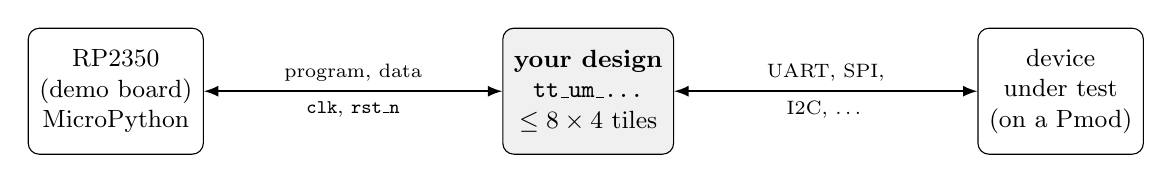
\begin{tikzpicture}[>=latex, box/.style={draw, rounded corners, align=center,
    minimum height=1.6cm, inner sep=4pt, font=\small}]
  \node[box] (host) at (0,0)
    {RP2350\\(demo board)\\MicroPython};
  \node[box, fill=gray!12] (chip) at (6,0)
    {\textbf{your design}\\\texttt{tt\_um\_\ldots}\\$\le 8\times4$ tiles};
  \node[box] (dev) at (12,0)
    {device\\under test\\(on a Pmod)};
  \draw[<->, thick] (host.east) -- node[above, font=\scriptsize]{program, data}
    node[below, font=\scriptsize]{\texttt{clk}, \texttt{rst\_n}} (chip.west);
  \draw[<->, thick] (chip.east) -- node[above, font=\scriptsize]{UART, SPI,}
    node[below, font=\scriptsize]{I2C, \ldots} (dev.west);
\end{tikzpicture}
\end{center}

\paragraph{Roadmap.} This lesson builds every layer you need, bottom up:
\begin{enumerate}[label=\arabic*.]
  \item the synchronous model of hardware, and why there is a clock
    (\cref{sec:sync,sec:timing});
  \item the outside world: metastability, synchronisers, reset
    (\cref{sec:meta,sec:reset});
  \item synthesisable Verilog, with a complete UART transmitter
    (\cref{sec:verilog});
  \item the protocols you must emulate, and what each demands from an
    architecture (\cref{sec:protocols});
  \item how the RP2040 PIO is built, with a working toy re-implementation
    (\cref{sec:pio});
  \item memories, the ASIC flow, area budgets (\cref{sec:memory,sec:flow});
  \item verification: simulation, reference models, formal proof
    (\cref{sec:verif});
  \item the design space for your own architecture, and a weekend-by-weekend
    plan (\cref{sec:design,sec:plan}).
\end{enumerate}
Every complete Verilog module in this lesson was compiled with Icarus
Verilog~13 and linted with Verilator~5.052. \texttt{uart\_tx},
\texttt{clkdiv}, \texttt{toy\_sm} and \texttt{crc\_serial} were also checked
by self-checking testbenches, the Python tests were run with cocotb~2.0.1, and
the formal properties were proven with SymbiYosys. \texttt{sync2} and the
Tiny Tapeout wrapper were compiled and linted only. All of it is teaching
code, not a finished design.

% ---------------------------------------------------------------------------
\subsection{The synchronous model: hardware as a step function}\label{sec:sync}

\paragraph{Motivation.} Software is a sequence of steps over time. Hardware is
a fixed set of physical wires and gates that all compute at once, all the
time. Designing directly in terms of analog voltages and delays is
intractable. The \emph{synchronous} discipline tames this: store all state in
registers that update only at one instant (the clock edge), and let
everything between registers be pure logic that has settled by then. Almost
every digital chip, including yours, is designed this way.

\begin{definition}[Combinational logic]
A circuit whose outputs are a function of its \emph{current} inputs only:
$y = f(x)$. It is built from gates (AND, OR, NOT, multiplexers, \ldots) with
no feedback loops. After the inputs change, the outputs are invalid
(``glitching'') for some propagation delay, and then settle to $f(x)$.
\end{definition}

\begin{definition}[Register, D flip-flop]
A D flip-flop has a data input $D$, a clock input, and an output $Q$. At each
rising clock edge it copies $D$ to $Q$; at all other times $Q$ holds its
value. An $n$-bit register is $n$ flip-flops sharing a clock.
\end{definition}

\begin{definition}[Synchronous circuit]
A circuit in which every flip-flop is clocked by the same clock, and every
loop in the wiring passes through at least one flip-flop. If the state
register holds $s$ and the inputs are $x$, then the circuit is fully
described by two combinational functions:
\[
  s_{t+1} = \delta(s_t, x_t), \qquad y_t = \lambda(s_t, x_t),
\]
where $t$ counts clock edges. This is a \emph{Mealy machine}. When the outputs
depend only on the state, $y_t=\lambda(s_t)$, it is a \emph{Moore machine}.
\end{definition}

\begin{center}
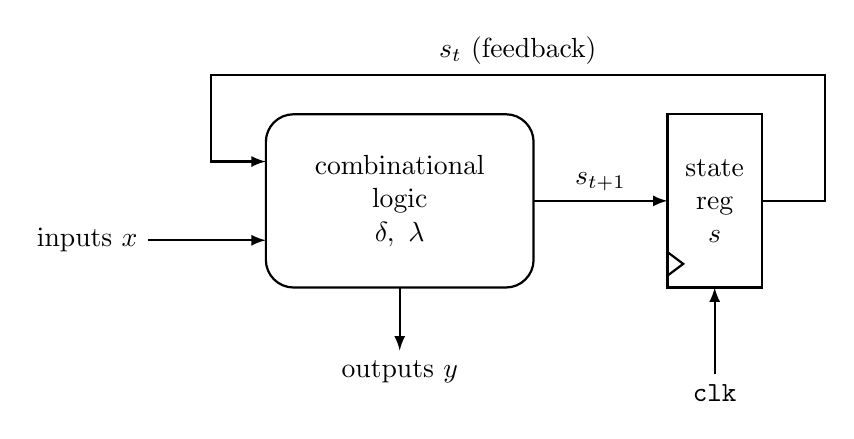
\begin{tikzpicture}[>=latex, thick]
  \node[draw, rounded corners=10pt, minimum width=3.4cm, minimum height=2.2cm,
    align=center] (f) at (0,0) {combinational\\logic\\$\delta,\ \lambda$};
  \node[draw, minimum width=1.2cm, minimum height=2.2cm, align=center]
    (r) at (4,0) {state\\reg\\$s$};
  \draw (3.4,-0.95) -- (3.6,-0.8) -- (3.4,-0.65);
  \draw[->] (-3.2,-0.5) node[left]{inputs $x$} -- (-1.7,-0.5);
  \draw[->] (1.7,0) -- node[above]{$s_{t+1}$} (3.4,0);
  \draw[->] (4.6,0) -- (5.4,0) -- (5.4,1.6) -- (-2.4,1.6) -- (-2.4,0.5)
    -- (-1.7,0.5);
  \node[above] at (1.5,1.6) {$s_t$ (feedback)};
  \draw[->] (0,-1.1) -- (0,-1.9) node[below]{outputs $y$};
  \draw[->] (4,-2.2) node[below]{\texttt{clk}} -- (4,-1.1);
\end{tikzpicture}
\end{center}

\begin{example}[A counter]
A 4-bit counter with enable $e$: $s_{t+1} = s_t + e_t \bmod 16$, and the
output is $y_t = s_t$. In Verilog:
\begin{verbatim}
reg [3:0] count;
always @(posedge clk) if (e) count <= count + 4'd1;
\end{verbatim}
Synthesis turns \texttt{count + 4'd1} into a small adder (pure logic) and
\texttt{count} into four flip-flops. The \texttt{if (e)} becomes a multiplexer
in front of each flip-flop, or a flip-flop with a built-in enable.
\end{example}

\begin{proposition}\label{prop:mealy}
Every synchronous circuit with $n$ flip-flops is a Mealy machine with at most
$2^n$ states. Conversely, every finite Mealy machine with $N$ states can be
implemented as a synchronous circuit with $\lceil\log_2 N\rceil$ flip-flops.
\end{proposition}
\begin{proof}
($\Rightarrow$) Cut every flip-flop out of the circuit. What remains has no
loops, because every loop passed through a flip-flop. So it is
combinational, and its outputs (the flip-flop $D$ inputs and the circuit
outputs) are functions of its inputs (the flip-flop $Q$ outputs and the
circuit inputs). Those functions are $\delta$ and $\lambda$, and the state
space is $\{0,1\}^n$.
($\Leftarrow$) Encode the states in binary with $\lceil\log_2 N\rceil$ bits.
Now $\delta$ and $\lambda$ are finite Boolean functions. Every Boolean
function can be built from AND, OR and NOT gates (for example from its
truth table, in sum-of-products form), and you place the flip-flops on the
state bits.
\end{proof}

\paragraph{The software analogy, and where it breaks.} A synchronous design
is a game loop: \texttt{state = step(state, inputs)}, run once per clock
edge, 60 million times a second at 60\,MHz. The analogy is good for
\emph{semantics}. It is bad for \emph{cost}, in three ways:
\begin{itemize}
  \item \textbf{Every line exists at once.} An \texttt{if/else} builds
    \emph{both} branches in silicon and a multiplexer picks one. A
    \texttt{for} loop is unrolled into copies of hardware. Nothing is
    ``executed''; it is all wired. You pay in area for everything you write,
    and in time only for the longest path.
  \item \textbf{All state updates are simultaneous.} Every register reads the
    \emph{old} state and writes the new one at the same instant, like
    double-buffering: compute the next frame from an immutable snapshot,
    then swap. Verilog's non-blocking assignment \texttt{<=} expresses this
    (see \cref{sec:verilog}).
  \item \textbf{No time inside a step.} There is no way to ``wait'' within
    a clock cycle. Waiting means staying in a state for many cycles, with a
    counter.
\end{itemize}

% ---------------------------------------------------------------------------
\subsection{Timing: why a clock has a maximum frequency}\label{sec:timing}

\paragraph{Motivation.} The synchronous model only holds if the logic between
registers has settled before the next edge. The rule that guarantees this
decides your maximum clock frequency. It also decides how much logic you may
chain within one cycle, and that is the deepest constraint on your
microarchitecture.

\begin{definition}[Flip-flop timing parameters]
For a flip-flop:
\begin{itemize}
  \item \emph{clock-to-Q delay} $t_{cq}$: time from the clock edge until $Q$
    shows the new value;
  \item \emph{setup time} $t_{su}$: $D$ must be stable for at least $t_{su}$
    \emph{before} the edge;
  \item \emph{hold time} $t_h$: $D$ must stay stable for at least $t_h$
    \emph{after} the edge.
\end{itemize}
If $D$ changes inside the window $[-t_{su}, +t_h]$ around the edge, the
flip-flop may become metastable (\cref{sec:meta}).
\end{definition}

\begin{center}
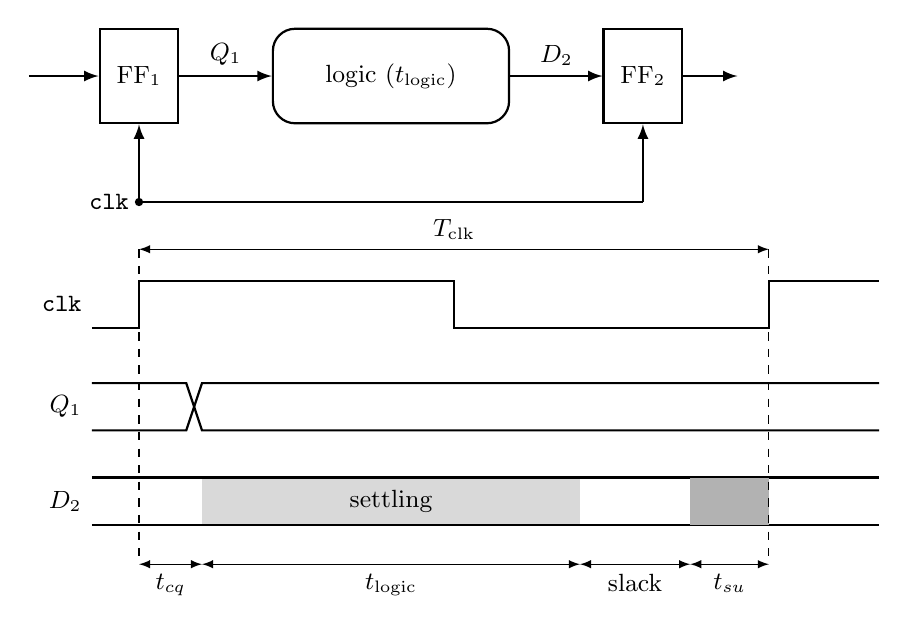
\begin{tikzpicture}[>=latex, thick, font=\small]
  % circuit
  \node[draw, minimum width=1cm, minimum height=1.2cm] (a) at (0,0) {FF$_1$};
  \node[draw, rounded corners=8pt, minimum width=3cm, minimum height=1.2cm]
    (l) at (3.2,0) {logic ($t_{\mathrm{logic}}$)};
  \node[draw, minimum width=1cm, minimum height=1.2cm] (b) at (6.4,0) {FF$_2$};
  \draw[->] (a.east) -- node[above]{$Q_1$} (l.west);
  \draw[->] (l.east) -- node[above]{$D_2$} (b.west);
  \draw[->] (-1.4,0) -- (a.west);
  \draw[->] (b.east) -- (7.6,0);
  \draw (0,-1.6) node[left]{\texttt{clk}} -- (6.4,-1.6);
  \draw[->] (0,-1.6) -- (a.south);
  \draw[->] (6.4,-1.6) -- (b.south);
  \fill (0,-1.6) circle (1.5pt);
  % waveform, edges at x = 0 and 8 (scaled 1.0)
  \begin{scope}[yshift=-3.2cm]
    \node[left] at (-0.6,0.3) {\texttt{clk}};
    \draw (-0.6,0) -- (0,0) -- (0,0.6) -- (4,0.6) -- (4,0) -- (8,0)
      -- (8,0.6) -- (9.4,0.6);
    \node[left] at (-0.6,-1.0) {$Q_1$};
    \draw (-0.6,-0.7) -- (0.6,-0.7) -- (0.8,-1.3) -- (9.4,-1.3);
    \draw (-0.6,-1.3) -- (0.6,-1.3) -- (0.8,-0.7) -- (9.4,-0.7);
    \node[left] at (-0.6,-2.2) {$D_2$};
    \fill[gray!30] (0.8,-1.9) rectangle (5.6,-2.5);
    \draw (-0.6,-1.9) -- (9.4,-1.9);
    \draw (-0.6,-2.5) -- (9.4,-2.5);
    \node at (3.2,-2.2) {settling};
    \fill[gray!60] (7.0,-1.9) rectangle (8,-2.5);
    % annotations
    \draw[<->, thin] (0,-3.0) -- node[below]{$t_{cq}$} (0.8,-3.0);
    \draw[<->, thin] (0.8,-3.0) -- node[below]{$t_{\mathrm{logic}}$} (5.6,-3.0);
    \draw[<->, thin] (5.6,-3.0) -- node[below]{slack} (7.0,-3.0);
    \draw[<->, thin] (7.0,-3.0) -- node[below]{$t_{su}$} (8,-3.0);
    \draw[<->, thin] (0,1.0) -- node[above]{$T_{\mathrm{clk}}$} (8,1.0);
    \draw[dashed, thin] (0,1.0) -- (0,-3.0);
    \draw[dashed, thin] (8,1.0) -- (8,-3.0);
  \end{scope}
\end{tikzpicture}
\end{center}

\begin{theorem}[Setup and hold constraints]\label{thm:timing}
Consider a path from flip-flop FF$_1$ through combinational logic to FF$_2$,
both on the same clock with period $T$. Let the clock arrive at FF$_2$ later
than at FF$_1$ by the skew $t_{\mathrm{skew}}$ (which may be negative). Then
the circuit behaves synchronously if
\begin{align}
  t_{cq} + t_{\mathrm{logic,max}} + t_{su} &\le T + t_{\mathrm{skew}},
    \label{eq:setup}\\
  t_{cq,\min} + t_{\mathrm{logic,min}} &\ge t_h + t_{\mathrm{skew}}.
    \label{eq:hold}
\end{align}
\end{theorem}
\begin{proof}
Measure time from the edge at FF$_1$. FF$_1$ launches new data that reaches
$D_2$ no later than $t_{cq}+t_{\mathrm{logic,max}}$. The next capturing edge
at FF$_2$ happens at $T+t_{\mathrm{skew}}$, and the data must be stable
$t_{su}$ before it, which gives~\eqref{eq:setup}. For hold: the \emph{same}
edge reaches FF$_2$ at time $t_{\mathrm{skew}}$, and FF$_2$ needs its old
$D_2$ stable until $t_{\mathrm{skew}}+t_h$. The fastest new data arrives at
$t_{cq,\min}+t_{\mathrm{logic,min}}$, which must not be earlier, and that
gives~\eqref{eq:hold}.
\end{proof}

Read the two inequalities as follows:
\begin{itemize}
  \item \textbf{Setup} violations mean ``too much logic for the clock
    period''. You fix them by a slower clock, less logic per cycle
    (pipelining), or faster cells. The longest register-to-register path is
    the \emph{critical path}, and $f_{\max} = 1/T_{\min}$ is set by it.
  \item \textbf{Hold} violations do not depend on $T$ at all, so slowing the
    clock never fixes them. The place-and-route tool fixes them by inserting
    delay buffers. That is one reason you leave area slack.
  \item The \emph{slack} of a path is how much earlier than required the
    data arrives. Static timing analysis (STA) checks every path in the
    netlist, at several process/voltage/temperature \emph{corners}, and
    reports the worst negative slack. You want all slacks $\ge 0$.
\end{itemize}

\begin{example}[Budgeting a 60\,MHz cycle]
At 60\,MHz, $T = 16.\overline{6}$\,ns. The numbers below are illustrative
only; read real ones from your STA report. Suppose $t_{cq}\approx0.4$\,ns,
$t_{su}\approx0.2$\,ns and the clock-tree skew is $0.3$\,ns against you.
That leaves about $15.7$\,ns for logic. With gates of roughly
$0.1$--$0.3$\,ns each in a 130\,nm process (depending on load and drive
strength), that is room for dozens of logic levels. A 32-bit adder plus a
few multiplexer levels fits comfortably. So at 60\,MHz your critical path is
usually not a single gate chain. It is more likely long wires, high fan-out
nets (one signal driving hundreds of inputs, like a global ``stall''), or a
chain such as decode $\to$ compare $\to$ select next PC $\to$ read
instruction memory.
\end{example}

\begin{remark}[One clock, and never logic on the clock]
Use exactly one clock, \texttt{clk}, for the whole design. To make something
happen at a slower rate, keep it on \texttt{clk} and gate its \emph{updates}
with an enable signal (\cref{sec:verilog}); this is how the PIO clock divider
works. Never divide the clock with a flip-flop and use the result as a
clock. Never put logic on a clock path. Never use a protocol signal (SPI's
SCK, I2C's SCL) as a clock. Such signals create new clock domains whose
skew the tools do not balance. Data crossing between domains needs the
synchronisers of \cref{sec:meta}, and gating logic on a clock glitches. In
your chip, \emph{protocol clocks are data}: you sample them on \texttt{clk}.
\end{remark}

% ---------------------------------------------------------------------------
\subsection{The asynchronous world: metastability and synchronisers}
\label{sec:meta}

\paragraph{Motivation.} \Cref{thm:timing} assumed that FF$_2$'s input comes
from your own clocked logic. Pin inputs do not. A UART RX line, an SPI clock
from an external controller, or an I2C line can change at any moment,
including inside a flip-flop's setup/hold window. A protocol emulator spends
its life sampling such signals, so this section is core material, not a
footnote.

\begin{definition}[Metastability]
If a flip-flop's $D$ changes inside its setup/hold window, its internal
latch can balance near the midpoint between 0 and 1 for an unbounded,
exponentially distributed time before resolving to a random value. While
metastable, $Q$ may be at an invalid voltage. Downstream gates may read it
inconsistently, some as 0 and some as 1.
\end{definition}

There is no software analogue of a bit that is neither 0 nor 1 for a while.
The nearest is a torn read of a variable being written by another thread,
but metastability happens even for a single bit.

\begin{proposition}[Synchroniser MTBF, standard model]
If asynchronous data with transition rate $f_d$ is sampled by a clock of
frequency $f_c$, and the sampled value is given a settling time $t_r$ before
anyone uses it, the mean time between failures is
\[
  \mathrm{MTBF} = \frac{e^{t_r/\tau}}{T_0\, f_c\, f_d},
\]
where $\tau$ and $T_0$ are properties of the flip-flop. Failure here means
still unresolved after $t_r$.
\end{proposition}
\begin{proof}[Proof sketch]
The chance that a given data transition lands in the critical window is
proportional to $T_0 f_c$ (window width times edge rate), so failures start
at rate $\propto T_0 f_c f_d$. The resolution of a metastable latch is a
linear instability with time constant $\tau$. So the probability that it
is still unresolved after $t_r$ falls like $e^{-t_r/\tau}$. MTBF is the
reciprocal of the product.
\end{proof}

The exponent is the whole point. One extra clock period of settling time
(at 60\,MHz, $t_r$ grows by about $16$\,ns, while $\tau$ is on the order of
tens of picoseconds) multiplies the MTBF by an astronomically large factor.
Hence:

\begin{definition}[Two-flop synchroniser]
Feed the asynchronous signal into a flip-flop, and feed that flip-flop into a
second one. Nothing else may read the first flip-flop. The second one's
output is safe to use in the \texttt{clk} domain.
\end{definition}

\begin{center}
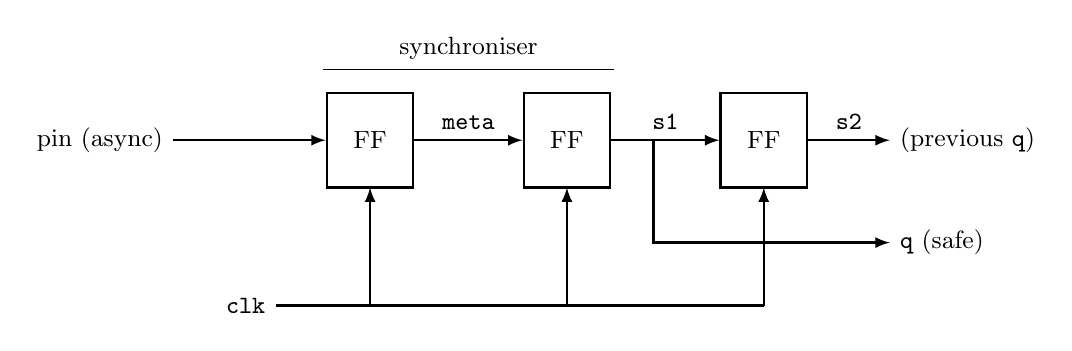
\begin{tikzpicture}[>=latex, thick, font=\small]
  \node[draw, minimum width=1.1cm, minimum height=1.2cm] (f1) at (2,0) {FF};
  \node[draw, minimum width=1.1cm, minimum height=1.2cm] (f2) at (4.5,0) {FF};
  \node[draw, minimum width=1.1cm, minimum height=1.2cm] (f3) at (7,0) {FF};
  \draw[->] (-0.5,0) node[left]{pin (async)} -- (f1.west);
  \draw[->] (f1.east) -- node[above]{\texttt{meta}} (f2.west);
  \draw[->] (f2.east) -- node[above]{\texttt{s1}} (f3.west);
  \draw[->] (f3.east) -- node[above]{\texttt{s2}} (8.6,0);
  \draw[->] (5.6,0) -- (5.6,-1.3) -- (8.6,-1.3) node[right]{\texttt{q} (safe)};
  \node[right] at (8.6,0) {(previous \texttt{q})};
  \draw (0.8,-2.1) node[left]{\texttt{clk}} -- (7,-2.1);
  \foreach \x in {2,4.5,7} \draw[->] (\x,-2.1) -- (\x,-0.6);
  \draw[thin] (1.4,0.9) -- (5.1,0.9);
  \node[above] at (3.25,0.9) {synchroniser};
\end{tikzpicture}
\end{center}

{\small
\begin{verbatim}
`default_nettype none
// Two-flop synchroniser plus rising/falling edge detector.
module sync2 (
    input  wire clk,
    input  wire d_async,   // straight from a pin: may change at any time
    output wire q,         // safe to use in the clk domain
    output wire rise,      // 1 for one cycle after q goes 0 -> 1
    output wire fall       // 1 for one cycle after q goes 1 -> 0
);
  reg meta, s1, s2;
  always @(posedge clk) begin
    meta <= d_async;   // may go metastable; never read it anywhere else
    s1   <= meta;      // has had a full cycle to settle
    s2   <= s1;        // previous value of s1, for edge detection
  end
  assign q    = s1;
  assign rise =  s1 & ~s2;
  assign fall = ~s1 &  s2;
endmodule
\end{verbatim}
}

\paragraph{Consequences for a protocol emulator.}
\begin{enumerate}[label=(\alph*)]
  \item \textbf{Latency.} An input change is visible to your logic two to
    three cycles after it happens at the pin, plus pad delay. Your response
    (driving an output) takes one more register plus output pad delay.
    The RP2040 PIO has exactly these synchronisers on every GPIO input
    (bypassable with \texttt{INPUT\_SYNC\_BYPASS}), and its documentation
    notes the two-cycle delay.
  \item \textbf{Target-mode speed limits.} When an external controller
    drives the clock (your chip as SPI \emph{target}), you detect its edges
    by sampling. Suppose that in SPI mode~0 you must change MISO after SCK
    falls and before the next rising edge. Your loop is: pin $\to$ 2
    synchroniser flops $\to$ edge detect $\to$ output register $\to$ pin.
    That is roughly 3--4 cycles of $16.7$\,ns plus about 10\,ns of pad
    delay, roughly 60--80\,ns. That must fit in half an SCK period, which
    caps SCK at a few MHz. This is my estimate; compute yours from your
    pipeline. A controller (your chip drives the clock) has no such limit,
    because you know when you will make the edge.
  \item \textbf{Multi-bit values.} Synchronising each bit of a bus separately
    can tear: if bits change together near an edge, some flops catch the new
    value and some the old, and the word you see never existed. Synchronise
    a single ``valid'' bit, or use a handshake, or Gray code for counters
    (exactly one bit changes per step).
  \item \textbf{Glitches and noise.} Slow edges, such as I2C's pull-up rise
    of up to $1\,\mu$s at 100\,kHz, can produce several apparent
    transitions. A digital filter (accept a new level only after it has
    been stable for $k$ samples) or majority voting over oversamples helps.
    A programmable filter is a useful general feature.
\end{enumerate}

\begin{remark}[Outputs must come from flip-flops]
The mirror rule for outputs: drive every protocol pin directly from a
flip-flop, never from combinational logic. Combinational outputs glitch while
they settle. A glitch on a data line is usually harmless, because the
receiver samples it at a defined time. A glitch on SCK, SCL or a chip select
is an extra edge, and it corrupts the transfer. Registered outputs also make
your output timing exactly predictable: the pin changes $t_{cq}$ plus pad
delay after the edge, every time.
\end{remark}

% ---------------------------------------------------------------------------
\subsection{Reset and initial state}\label{sec:reset}

The post warns about this: ``Unlike an FPGA, flops don't start at 0, so your
design needs to use the reset signal (\texttt{rst\_n}) to get into a known
state.'' On an FPGA, the bitstream initialises every flip-flop, so Verilog
\texttt{initial} values and \texttt{reg x = 0;} work. On an ASIC a
flip-flop powers up as 0 or 1 at random, and synthesis cannot implement
initial values. Everything that matters must be reset explicitly.

\begin{itemize}
  \item \textbf{Synchronous reset} (\texttt{always @(posedge clk) if
    (!rst\_n) \ldots}) treats reset like any other input to the next-state
    logic. It needs the clock running during reset. It is simple and is the
    style of the TT examples. I use it throughout.
  \item \textbf{Asynchronous reset} (\texttt{always @(posedge clk or negedge
    rst\_n)}) uses flip-flops with a reset pin, so it works without a clock.
    Its \emph{release} must still be synchronised to \texttt{clk}.
    Otherwise some flops leave reset one cycle before others and the state
    is inconsistent.
  \item \texttt{rst\_n} comes from a microcontroller pin, asynchronous to
    \texttt{clk} unless you know otherwise. Pass it through a two-flop
    synchroniser before use, as with any other input.
  \item \textbf{What does not need reset?} Pure data registers such as
    memory contents, shift-register data or FIFO storage, as long as control
    state (valid bits, pointers, the PC) is reset so the garbage is never
    used. Fewer resets means less area and less routing.
  \item TT detail from the post: when your design is deselected it is
    powered down and loses state. Your program must be reloaded after it is
    reselected. Design the loader with that in mind.
\end{itemize}

Gate-level simulation is where reset bugs show up. In RTL simulation, an
\texttt{if (x)} whose condition is the unknown value \texttt{X} quietly takes
the \texttt{else} branch (``X-optimism''). The gate-level netlist propagates
\texttt{X} faithfully, so an unreset register poisons everything downstream.

% ---------------------------------------------------------------------------
\subsection{Verilog that synthesises}\label{sec:verilog}

\paragraph{Motivation.} Verilog was designed as a \emph{simulation} language,
and synthesis tools accept only a subset of it, interpreted as hardware. Much
legal Verilog either does not synthesise or synthesises into something other
than what simulation showed. You already know modules and ports. This
section is the field guide to the rest.

\subsubsection{Two kinds of \texttt{always} block}

\begin{definition}[The two synthesisable process styles]
\begin{enumerate}[label=(\roman*)]
  \item \textbf{Sequential}: \texttt{always @(posedge clk)}, using only
    non-blocking assignments \texttt{<=}. Every variable assigned here
    becomes a flip-flop.
  \item \textbf{Combinational}: \texttt{always @*} (or \texttt{assign}),
    using only blocking assignments \texttt{=}. Every variable must be
    assigned on \emph{every} path through the block. It becomes pure logic.
\end{enumerate}
Never mix the two assignment kinds in one block, and never assign one
variable from two blocks (that is a multiple-driver error: two pieces of
hardware fighting over one wire).
\end{definition}

\paragraph{Why \texttt{<=} in sequential blocks.} The simulator handles a
non-blocking assignment by evaluating the right-hand side now and deferring
the update to the end of the current time step. Every \texttt{<=} in the
design therefore reads \emph{pre-edge} values, which is exactly the
flip-flop semantics of \cref{sec:sync}. Compare:
\begin{verbatim}
always @(posedge clk) begin a <= b; b <= a; end  // swaps a and b
always @(posedge clk) begin a =  b; b =  a; end  // both end up equal to b
\end{verbatim}
Worse, with \texttt{=}, two \emph{different} \texttt{always @(posedge clk)}
blocks that read each other's variables give a result that depends on which
block the simulator happens to run first. That is a race, and synthesis
will build something that matches neither ordering. The analogy is
computing a whole frame from an immutable snapshot (\texttt{<=}) versus
mutating shared state in place (\texttt{=}).

\paragraph{A useful consequence: last assignment wins.} Within one block, if
several \texttt{<=} to the same variable execute in the same cycle, the last
one takes effect. This gives clean priority logic:
\begin{verbatim}
always @(posedge clk) begin
  if (shift)  out <= data[0];
  if (force)  out <= force_val;   // overrides shift when both are true
end
\end{verbatim}

\subsubsection{Latches: the classic combinational bug}

If a combinational block fails to assign a variable on some path, the
variable must \emph{remember} its old value on that path. Remembering without
a clock is a \emph{latch}: a level-sensitive storage element. Here it is
almost always a bug: it is a timing hazard and invisible in your mental
model.
\begin{verbatim}
always @* begin                 // BUG: no assignment when sel is 2 or 3
  case (sel)
    2'd0: y = a;
    2'd1: y = b;
  endcase
end
\end{verbatim}
Both tools flag it (module name \texttt{latchy}):
\begin{verbatim}
yosys:     Warning: Latch inferred for signal `\latchy.\y' ...
verilator: %Warning-LATCH: Latch inferred for signal 'y' ...
\end{verbatim}
The fix is to give every output a default at the top of the block, then
override it:
\begin{verbatim}
always @* begin
  y = 1'b0;                     // default first
  case (sel)
    2'd0: y = a;
    2'd1: y = b;
    default: ;
  endcase
end
\end{verbatim}

\subsubsection{Other rules worth memorising}
\begin{itemize}
  \item \textbf{\texttt{`default\_nettype none}} at the top of every file
    (the TT template does this). Without it, a misspelled signal name
    silently becomes a new 1-bit wire.
  \item \textbf{Widths.} Verilog silently truncates and zero-extends.
    Unsized literals like \texttt{1} are 32 bits. \texttt{a + b} of two 8-bit
    values assigned to an 8-bit result drops the carry. If one operand is
    unsigned the whole expression is unsigned, so \texttt{\$signed}
    comparisons go wrong silently. Size your constants (\texttt{4'd1}) and
    let Verilator's \texttt{-Wall} lint complain about every width mismatch.
  \item \textbf{Not synthesisable:} \texttt{\#} delays, \texttt{initial}
    blocks (on an ASIC; \cref{sec:reset}), \texttt{\$display} and other
    system tasks (simulation only), \texttt{real}, loops whose bound is not
    a compile-time constant. \texttt{for} with a constant bound is fine; it
    unrolls into copies of hardware.
  \item \textbf{Memories.} \texttt{reg [15:0] mem [0:31];} synthesises to
    flip-flops plus read multiplexers on an ASIC. Synthesis will never turn
    it into an SRAM macro by itself; you instantiate macros explicitly
    (\cref{sec:memory}).
  \item \textbf{\texttt{parameter} and \texttt{generate}} are compile-time
    metaprogramming, like const generics: they set widths and replicate
    hardware (e.g.\ $N$ state machines) at elaboration time.
  \item \textbf{Clock enables, not derived clocks.} A slow process is
    \texttt{always @(posedge clk) if (en) \ldots}, where \texttt{en} is a
    one-cycle pulse from a counter.
\end{itemize}

\subsubsection{Valid/ready handshakes}

Most blocks exchange data with a two-signal handshake. The producer drives
\texttt{data} and \texttt{valid}; the consumer drives \texttt{ready}; a
transfer happens on every clock edge where \texttt{valid \&\& ready}. This is
backpressure, like a bounded channel in Rust: the producer must hold
\texttt{data} and \texttt{valid} stable until the transfer happens. The
host-to-engine FIFOs of a PIO use this protocol.

\subsubsection{Worked example: a UART transmitter}\label{sec:uarttx}

UART framing is covered in \cref{sec:uart}. In short: the line idles high,
and a byte is sent as a 0 start bit, eight data bits LSB first, and a 1 stop
bit, each lasting $f_{\mathrm{clk}}/\text{baud}$ clock cycles.
{\small
\begin{verbatim}
`default_nettype none
// Fixed-function 8N1 UART transmitter. CLKS_PER_BIT = f_clk / baud.
module uart_tx #(
    parameter CLKS_PER_BIT = 521          // 60 MHz / 115200 = 520.8
) (
    input  wire       clk,
    input  wire       rst_n,
    input  wire [7:0] data,
    input  wire       valid,              // host has a byte for us
    output wire       ready,              // we can take it this cycle
    output reg        tx
);
  localparam CW = $clog2(CLKS_PER_BIT);
  reg [CW-1:0] baud_cnt;                  // clocks left in current bit
  reg [3:0]    bit_idx;                   // 0 = start, 1..8 = data, 9 = stop
  reg [7:0]    shreg;
  reg          busy;

  assign ready = !busy;

  always @(posedge clk) begin
    if (!rst_n) begin
      tx <= 1'b1;                         // idle line is high
      busy <= 1'b0;
      baud_cnt <= 0;
      bit_idx <= 0;
      shreg <= 0;
    end else if (!busy) begin
      if (valid) begin                    // handshake: valid && ready
        shreg    <= data;
        busy     <= 1'b1;
        tx       <= 1'b0;                 // start bit
        bit_idx  <= 0;
        baud_cnt <= CLKS_PER_BIT - 1;
      end
    end else if (baud_cnt != 0) begin
      baud_cnt <= baud_cnt - 1'b1;
    end else begin                        // end of a bit period
      baud_cnt <= CLKS_PER_BIT - 1;
      bit_idx  <= bit_idx + 1'b1;
      if (bit_idx < 8) begin              // next: data bit bit_idx (LSB first)
        tx    <= shreg[0];
        shreg <= shreg >> 1;
      end else if (bit_idx == 8) begin
        tx <= 1'b1;                       // stop bit
      end else begin
        busy <= 1'b0;                     // stop bit finished
      end
    end
  end
endmodule
\end{verbatim}
}
Points to notice:
\begin{itemize}
  \item The counter is loaded with \texttt{CLKS\_PER\_BIT - 1} and counts
    down to 0, so a bit lasts exactly \texttt{CLKS\_PER\_BIT} cycles: the loaded value
    plus the cycle spent at 0. Off-by-one errors in counters are the most
    common bug in this kind of code, so the testbench checks the width of
    every bit, cycle by cycle.
  \item \texttt{tx} is a register (\cref{sec:meta}: outputs from flops).
  \item Back to back, the stop bit lasts one extra cycle, because
    \texttt{busy} drops and the next byte is accepted on the following edge.
    UART allows stop bits longer than one bit time, so this is legal. A
    tighter design would accept the next byte in the last stop-bit cycle.
  \item The design is a Moore machine: its state is (\texttt{busy},
    \texttt{bit\_idx}, \texttt{baud\_cnt}, \texttt{shreg}, \texttt{tx}).
\end{itemize}

\paragraph{Wrapping it for Tiny Tapeout.} The TT top module has a fixed port
list (from the template's \texttt{src/project.v}). Its name must start with
\texttt{tt\_um\_}, every output must be driven, and \texttt{uio\_oe} bit
$i=1$ makes \texttt{uio[$i$]} an output. The recommended-pinouts page lists
\texttt{uo\_out[4]} as UART TX (and \texttt{ui\_in[3]} as RX) for UART to USB
through the demo board's microcontroller.
{\small
\begin{verbatim}
`default_nettype none
// Milestone 1: endlessly transmit the byte set on the DIP switches.
module tt_um_kaarlo_uart (
    input  wire [7:0] ui_in,
    output wire [7:0] uo_out,
    input  wire [7:0] uio_in,
    output wire [7:0] uio_out,
    output wire [7:0] uio_oe,
    input  wire       ena,
    input  wire       clk,
    input  wire       rst_n
);
  // Switches are asynchronous to clk: synchronise before use.
  reg [7:0] sw_meta, sw;
  always @(posedge clk) begin
    sw_meta <= ui_in;
    sw      <= sw_meta;
  end

  wire tx, ready;
  uart_tx #(.CLKS_PER_BIT(521)) u_tx (   // 115200 baud at 60 MHz
      .clk(clk), .rst_n(rst_n),
      .data(sw), .valid(1'b1), .ready(ready), .tx(tx)
  );

  assign uo_out  = {3'b000, tx, 4'b0000};  // TX on uo_out[4]
  assign uio_out = 8'h00;
  assign uio_oe  = 8'h00;                  // all bidirectional pins are inputs

  wire _unused = &{ena, uio_in, ready, 1'b0};
endmodule
\end{verbatim}
}
Per-bit synchronisation of \texttt{ui\_in} can tear (\cref{sec:meta}(c)).
For hand-flipped switches that only means one wrong byte while a switch
moves. For a real data bus from the host, it is not acceptable: synchronise
a strobe and sample the bus once it has been stable. Also,
\texttt{rst\_n} is used here without a synchroniser, which is acceptable for
a first experiment but not for the real design (\cref{sec:reset}).

% ---------------------------------------------------------------------------
\subsection{The protocols, and what they demand}\label{sec:protocols}

\paragraph{Motivation.} You cannot design a general architecture until you
know what the protocols have in common and where they differ. For each
protocol below, note three things: who owns the timing, which pins change
direction, and which per-bit work (counting, CRC, stuffing) recurs.
\Cref{tab:needs} at the end of the section collects them.

\subsubsection{UART}\label{sec:uart}

\begin{center}
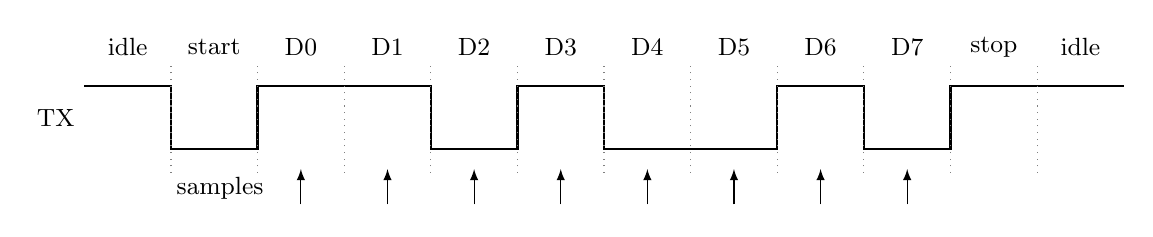
\begin{tikzpicture}[>=latex, font=\small]
  \draw[thick] (0,0.8) -- (1.1,0.8) -- (1.1,0) -- (2.2,0) -- (2.2,0.8) -- (4.4,0.8) -- (4.4,0) -- (5.5,0) -- (5.5,0.8) -- (6.6,0.8) -- (6.6,0) -- (8.8,0) -- (8.8,0.8) -- (9.9,0.8) -- (9.9,0) -- (11,0) -- (11,0.8) -- (13.2,0.8);
  \foreach \x in {1.1,2.2,...,12.1} \draw[gray, dotted] (\x,-0.3) -- (\x,1.1);
  \node at (0.55,1.3) {idle};
  \node at (1.65,1.3) {start};
  \foreach \i in {0,...,7} \node at ({2.75+1.1*\i},1.3) {D\i};
  \node at (11.55,1.3) {stop};
  \node at (12.65,1.3) {idle};
  \foreach \i in {0,...,7} \draw[->, thin] ({2.75+1.1*\i},-0.7) -- ({2.75+1.1*\i},-0.25);
  \node[left] at (0,0.4) {TX};
  \node[left] at (2.4,-0.5) {samples};
\end{tikzpicture}
\end{center}
The byte above is \texttt{0x4B} $=0100\,1011_2$, sent LSB first:
1,1,0,1,0,0,1,0. Variants: 5--9 data bits, optional parity bit (even/odd)
before the stop bit, 1 or 2 stop bits. ``8N1'' is 8 data, no parity, 1 stop.
Each side has its own clock, and the receiver resynchronises only on the
start bit's falling edge.

\paragraph{Receiving.} Wait for a falling edge (after the synchroniser), wait
1.5 bit times to land in the middle of D0, then sample every bit time.
Robust receivers oversample at $16\times$ and majority-vote three samples
around the bit centre. They also check that the start bit is still low at
its middle (rejecting glitches) and that the stop bit is high (a framing
error otherwise). A line held low for a whole frame is a \emph{break}.

\begin{proposition}[UART clock tolerance]\label{prop:baud}
Let the transmitter's bit time be $T$ and the receiver's $T(1+\delta)$. Let
the receiver detect the start edge with a lag $\varepsilon\in[0,\varepsilon_{\max}]$
and sample bit $k$ ($k=0$ the start bit, $k=9$ the stop bit of 8N1) at time
$(k+\tfrac12)T(1+\delta)+\varepsilon$ after the true edge. All samples land
inside their bits if
\[
  -\frac{1}{19} < \delta \quad\text{and}\quad
  \delta < \frac{1/2 - \varepsilon_{\max}/T}{9.5}.
\]
In particular, with $\varepsilon=0$, $|\delta| < 1/19 \approx 5.3\%$.
\end{proposition}
\begin{proof}
Bit $k$ occupies $[kT,(k+1)T)$. The sample time grows with $k$ when
$\delta>-1$, so the worst cases are at the last sample $k=9$. Lower bound
(receiver too fast, $\delta<0$, $\varepsilon=0$): we need
$9.5T(1+\delta) \ge 9T$, i.e.\ $\delta \ge -1/19$. Upper bound (receiver too
slow, $\delta>0$, lag $\varepsilon_{\max}$): we need
$9.5T(1+\delta)+\varepsilon_{\max} < 10T$, which rearranges to the stated
bound. For $k<9$ the same inequalities with $k+\tfrac12<9.5$ are weaker.
\end{proof}
With $16\times$ oversampling $\varepsilon_{\max}\approx T/16$, giving about
$4.6\%$ in total, which is usually split as about $2\%$ per side. With a
60\,MHz clock and an integer divider:
\begin{center}
\begin{tabular}{|r|r|r|r|}
\hline
baud & $60\,\mathrm{MHz}/\text{baud}$ & integer divider & error \\ \hline
9600 & 6250 & 6250 & 0 \\
115200 & 520.83 & 521 & $-0.03\%$ (slightly slow) \\
921600 & 65.10 & 65 & $+0.16\%$ \\
1000000 & 60 & 60 & 0 \\
3000000 & 20 & 20 & 0 \\ \hline
\end{tabular}
\end{center}
At 60\,MHz, an integer divider is accurate enough for every common baud
rate. A fractional divider (\cref{sec:pio}) mostly matters at low
oversampling ratios or odd clocks.

\subsubsection{SPI}

A controller drives SCK, MOSI (controller out, target in) and an active-low
chip select CS. The target drives MISO. Data is usually MSB first, in words
of 8 bits or more. Two bits configure the clock:
CPOL is the idle level of SCK, and CPHA says whether data is sampled on the
leading (CPHA$=0$) or trailing (CPHA$=1$) edge of each pulse. The other edge
is when data changes.
\begin{center}
\begin{tabular}{|c|c|c|l|l|}
\hline
mode & CPOL & CPHA & SCK idle & sample edge \\ \hline
0 & 0 & 0 & low & rising (leading) \\
1 & 0 & 1 & low & falling (trailing) \\
2 & 1 & 0 & high & falling (leading) \\
3 & 1 & 1 & high & rising (trailing) \\ \hline
\end{tabular}
\end{center}
\begin{center}
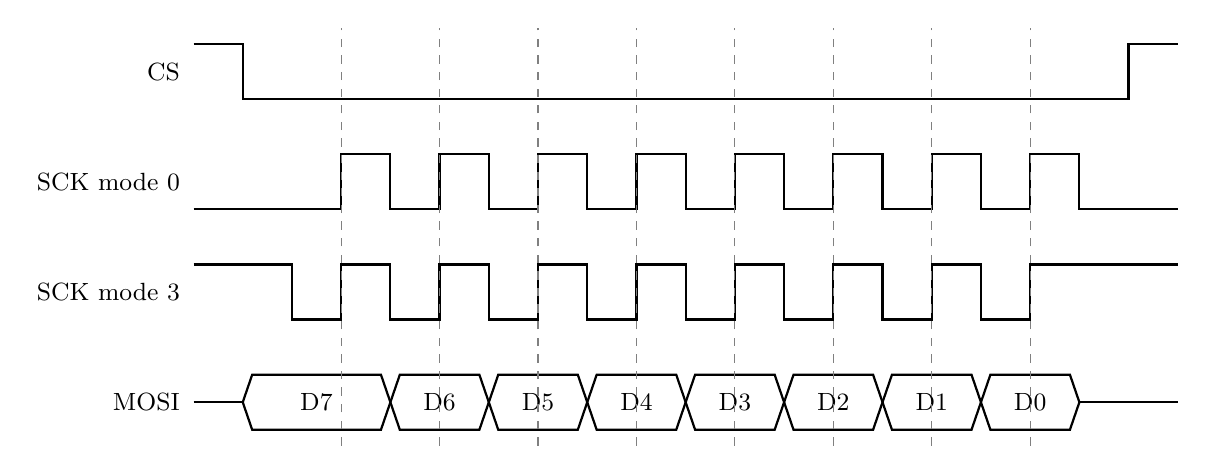
\begin{tikzpicture}[>=latex, font=\small]
  \draw[thick] (-1.25,4.9) -- (-0.625,4.9) -- (-0.625,4.2) -- (10.625,4.2) -- (10.625,4.9) -- (11.25,4.9);
  \draw[thick] (-1.25,2.8) -- (0.625,2.8) -- (0.625,3.5) -- (1.25,3.5) -- (1.25,2.8) -- (1.875,2.8) -- (1.875,3.5) -- (2.5,3.5) -- (2.5,2.8) -- (3.125,2.8) -- (3.125,3.5) -- (3.75,3.5) -- (3.75,2.8) -- (4.375,2.8) -- (4.375,3.5) -- (5,3.5) -- (5,2.8) -- (5.625,2.8) -- (5.625,3.5) -- (6.25,3.5) -- (6.25,2.8) -- (6.875,2.8) -- (6.875,3.5) -- (7.5,3.5) -- (7.5,2.8) -- (8.125,2.8) -- (8.125,3.5) -- (8.75,3.5) -- (8.75,2.8) -- (9.375,2.8) -- (9.375,3.5) -- (10,3.5) -- (10,2.8) -- (11.25,2.8);
  \draw[thick] (-1.25,2.1) -- (0,2.1) -- (0,1.4) -- (0.625,1.4) -- (0.625,2.1) -- (1.25,2.1) -- (1.25,1.4) -- (1.875,1.4) -- (1.875,2.1) -- (2.5,2.1) -- (2.5,1.4) -- (3.125,1.4) -- (3.125,2.1) -- (3.75,2.1) -- (3.75,1.4) -- (4.375,1.4) -- (4.375,2.1) -- (5,2.1) -- (5,1.4) -- (5.625,1.4) -- (5.625,2.1) -- (6.25,2.1) -- (6.25,1.4) -- (6.875,1.4) -- (6.875,2.1) -- (7.5,2.1) -- (7.5,1.4) -- (8.125,1.4) -- (8.125,2.1) -- (8.75,2.1) -- (8.75,1.4) -- (9.375,1.4) -- (9.375,2.1) -- (11.25,2.1);
  % MOSI as a bus
  \draw[thick] (-1.25,0.35) -- (-0.625,0.35);
  \draw[thick] (-0.625,0.35) -- (-0.505,0.7) -- (1.13,0.7) -- (1.25,0.35)
    -- (1.13,0) -- (-0.505,0) -- cycle;
  \node at (0.31,0.35) {D7};
  \foreach \k/\lab in {1/D6,2/D5,3/D4,4/D3,5/D2,6/D1,7/D0} {
    \draw[thick] ({1.25*\k},0.35) -- ({1.25*\k+0.12},0.7)
      -- ({1.25*\k+1.13},0.7) -- ({1.25*\k+1.25},0.35)
      -- ({1.25*\k+1.13},0) -- ({1.25*\k+0.12},0) -- cycle;
    \node at ({1.25*\k+0.625},0.35) {\lab};
  }
  \draw[thick] (10,0.35) -- (11.25,0.35);
  \foreach \k in {0,...,7} \draw[gray, dashed] ({1.25*\k+0.625},-0.2) -- ({1.25*\k+0.625},5.1);
  \node[left] at (-1.3,4.55) {CS};
  \node[left] at (-1.3,3.15) {SCK mode 0};
  \node[left] at (-1.3,1.75) {SCK mode 3};
  \node[left] at (-1.3,0.35) {MOSI};
\end{tikzpicture}
\end{center}
Dashed lines are the sample instants. In modes 0 and 3 both sample on rising
edges, and the waveforms differ only in the idle level. In mode~0 the first
bit must already be valid when CS falls, because the first edge is a
sampling edge. MISO looks like MOSI but is driven by the target. Note how
little a controller needs: drive two outputs on one edge, sample one input
on the other. It is the easiest protocol to make fast. Being a \emph{target}
is harder (\cref{sec:meta}(b)).

\subsubsection{I2C}

I2C uses two \emph{open-drain} lines, SCL and SDA, each pulled up by a
resistor. A device can only pull a line low or let go of it. Nobody ever
drives high. This makes the bus a wired-AND: the line is high only if every
device lets go. Arbitration, acknowledgement and clock stretching are all
built on this.
\begin{center}
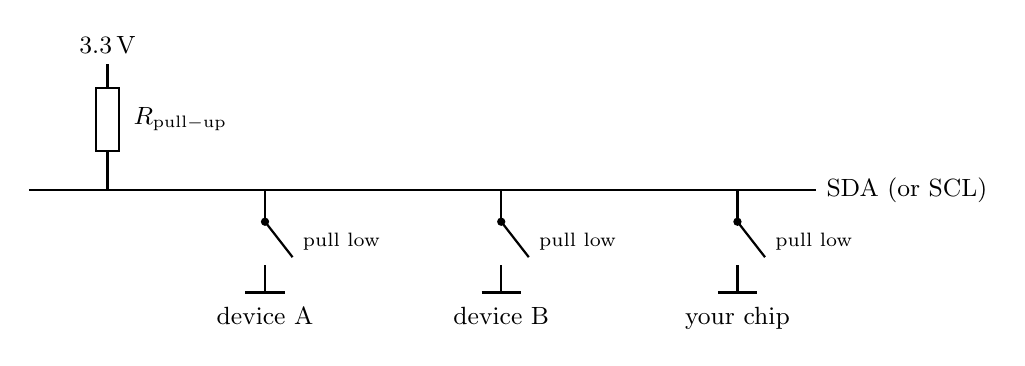
\begin{tikzpicture}[>=latex, font=\small, thick]
  \draw (0,2.2) node[above]{3.3\,V} -- (0,1.9);
  \draw (-0.15,1.9) rectangle (0.15,1.1);
  \node[right] at (0.2,1.5) {$R_{\mathrm{pull\text{-}up}}$};
  \draw (0,1.1) -- (0,0.6);
  \draw (-1,0.6) -- (9,0.6) node[right]{SDA (or SCL)};
  \foreach \x/\lab in {2/device A,5/device B,8/your chip} {
    \draw (\x,0.6) -- (\x,0.2);
    \draw (\x,0.2) -- (\x+0.35,-0.25);
    \fill (\x,0.2) circle (1.5pt);
    \draw (\x,-0.35) -- (\x,-0.7);
    \draw (\x-0.25,-0.7) -- (\x+0.25,-0.7);
    \node[below] at (\x,-0.75) {\lab};
    \node[right, font=\scriptsize] at (\x+0.35,-0.05) {pull low};
  }
\end{tikzpicture}
\end{center}
\begin{center}
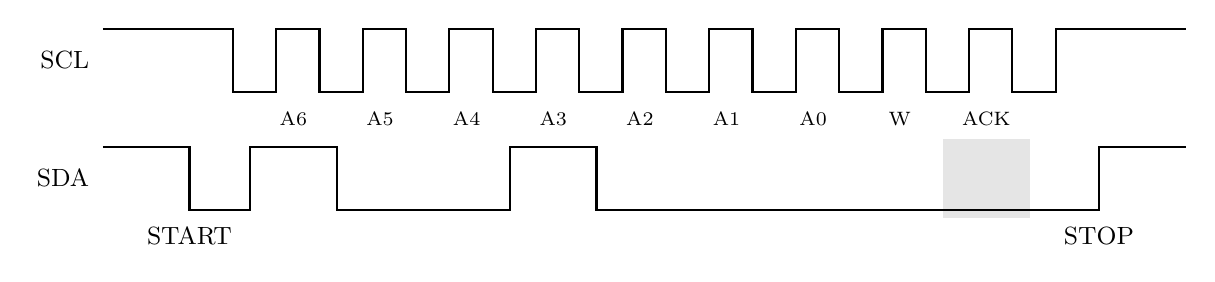
\begin{tikzpicture}[>=latex, font=\small]
  \fill[gray!20] (10.12,-0.1) rectangle (11.22,0.9);
  \draw[thick] (-0.55,2.3) -- (1.1,2.3) -- (1.1,1.5) -- (1.65,1.5) -- (1.65,2.3) -- (2.2,2.3) -- (2.2,1.5) -- (2.75,1.5) -- (2.75,2.3) -- (3.3,2.3) -- (3.3,1.5) -- (3.85,1.5) -- (3.85,2.3) -- (4.4,2.3) -- (4.4,1.5) -- (4.95,1.5) -- (4.95,2.3) -- (5.5,2.3) -- (5.5,1.5) -- (6.05,1.5) -- (6.05,2.3) -- (6.6,2.3) -- (6.6,1.5) -- (7.15,1.5) -- (7.15,2.3) -- (7.7,2.3) -- (7.7,1.5) -- (8.25,1.5) -- (8.25,2.3) -- (8.8,2.3) -- (8.8,1.5) -- (9.35,1.5) -- (9.35,2.3) -- (9.9,2.3) -- (9.9,1.5) -- (10.45,1.5) -- (10.45,2.3) -- (11,2.3) -- (11,1.5) -- (11.55,1.5) -- (11.55,2.3) -- (13.2,2.3);
  \draw[thick] (-0.55,0.8) -- (0.55,0.8) -- (0.55,0) -- (1.32,0) -- (1.32,0.8) -- (2.42,0.8) -- (2.42,0) -- (4.62,0) -- (4.62,0.8) -- (5.72,0.8) -- (5.72,0) -- (12.1,0) -- (12.1,0.8) -- (13.2,0.8);
  \node[left] at (-0.6,1.9) {SCL};
  \node[left] at (-0.6,0.4) {SDA};
  \node[below] at (0.55,-0.1) {START};
  \node[below] at (12.1,-0.1) {STOP};
  \foreach \i/\lab in {0/A6,1/A5,2/A4,3/A3,4/A2,5/A1,6/A0,7/W,8/ACK}
    \node[font=\scriptsize] at ({1.1*(1.7+\i)},1.15) {\lab};
\end{tikzpicture}
\end{center}
A write to 7-bit address \texttt{0x48}. The rules:
\begin{itemize}
  \item SDA may change only while SCL is low. SDA falling while SCL is high
    is START; SDA rising while SCL is high is STOP. A START without a
    preceding STOP is a \emph{repeated start}.
  \item After START: 7 address bits MSB first and a R/$\overline{\text{W}}$
    bit (1 = read), then a 9th clock in which the \emph{receiver} pulls SDA
    low to ACK (shaded; the target drives it here). High in the 9th clock is
    NACK. Data bytes follow, each with its own ACK.
  \item \textbf{Clock stretching}: a target may hold SCL low to make the
    controller wait. A controller must therefore release SCL and then
    \emph{wait until it actually reads high}, rather than assume it.
  \item Speeds: standard mode 100\,kHz (minimum SCL low time $4.7\,\mu$s,
    high time $4.0\,\mu$s), fast mode 400\,kHz ($1.3\,\mu$s low,
    $0.6\,\mu$s high). Rise time is set by the pull-up and bus capacitance
    (at most 1000\,ns and 300\,ns respectively), which is why you need
    synchronised, possibly filtered reads.
\end{itemize}
\paragraph{Open drain on Tiny Tapeout.} The pads have no open-drain mode, but
you can emulate one with a bidirectional pin: tie its output value to 0 and
toggle the output enable.
\begin{verbatim}
assign uio_out[3] = 1'b0;        // when driving, drive low
assign uio_oe[3]  = sda_pull;    // 1 = pull low, 0 = release (pulled up)
// read the real bus level through a synchroniser from uio_in[3]
\end{verbatim}
Never set \texttt{uio\_oe} with a 1 output on an I2C line. That drives high
against a device pulling low, which is a short circuit through two
transistors. The pull-ups are external, on the Pmod or the device board.
The recommended TT pinout puts SCL/SDA on \texttt{uio[2]}/\texttt{uio[3]}
(top Pmod row) or \texttt{uio[6]}/\texttt{uio[7]} (bottom row).

\subsubsection{The other suggested protocols, briefly}
\begin{itemize}
  \item \textbf{JTAG}: TCK, TMS, TDI from the controller, TDO from the
    target. The target samples TMS and TDI on TCK's rising edge and changes
    TDO on the falling edge. TMS steers a fixed 16-state TAP state machine;
    long shift chains go through TDI$\to$TDO. Easy timing, long bit
    sequences.
  \item \textbf{SWD} (ARM): one clock and one \emph{bidirectional} data
    line, with turnaround cycles where neither side drives. The line
    switches direction in the middle of a transaction, with a 3-bit ACK and
    a parity bit. This tests whether your engine can change a pin's
    direction on an exact cycle (PIO does this with side-set on pin
    directions).
  \item \textbf{PS/2}: open-drain clock and data, with the \emph{device}
    generating the clock (roughly 10--16.7\,kHz). Frames are 11 bits: start
    0, 8 data LSB first, odd parity, stop 1. The host requests to send by
    holding clock low. This tests external-clock following and
    open-drain handling.
  \item \textbf{CAN}: one logical line through an external transceiver, with
    dominant (0) and recessive (1) states. That is wired-AND again, so
    bitwise arbitration works: a node that sends recessive but reads
    dominant has lost and stops sending. After five equal bits, a
    complement bit is stuffed. The CRC is 15 bits. Receivers resynchronise
    their bit timing on edges, and the sample point sits late in the bit.
    This tests reading back what you transmit, every bit, and edge-driven
    phase adjustment.
\end{itemize}

\subsubsection{Low-speed USB (stretch goal)}
Low-speed USB runs at 1.5\,Mbit/s on a differential pair D+/D$-$, which is
40 clock cycles per bit at 60\,MHz. A low-speed device announces itself with a
1.5\,k$\Omega$ pull-up on D$-$. The line code combines several ideas worth
building as general hardware:
\begin{itemize}
  \item \textbf{NRZI}: a 0 is a \emph{transition}, a 1 is \emph{no change}.
  \item \textbf{Bit stuffing}: after six consecutive 1s the transmitter
    inserts a 0, which forces a transition so the receiver can stay locked.
    The receiver deletes it.
  \item \textbf{SE0}: both lines low, which is neither J nor K. Two bit times
    of SE0 then J mark end-of-packet. Packets begin with a SYNC pattern.
  \item \textbf{CRCs}: CRC-5 on tokens, CRC-16 on data.
  \item \textbf{Turnaround}: a device must start replying within a small,
    fixed number of bit times. Check the bus-turnaround timing in chapter~7
    of the USB~2.0 specification.
\end{itemize}
\begin{center}
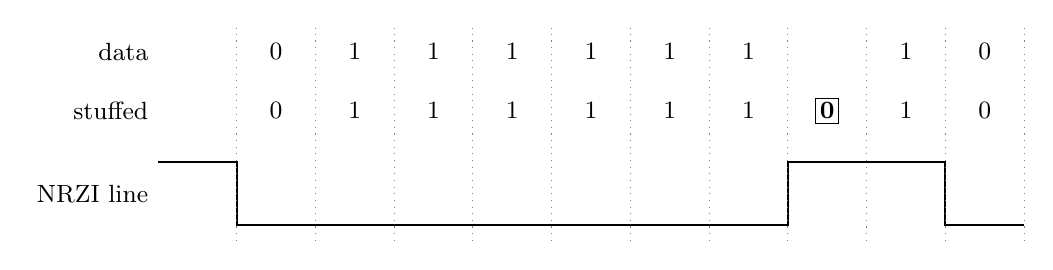
\begin{tikzpicture}[>=latex, font=\small]
  \draw[thick] (-1,0.8) -- (0,0.8) -- (0,0) -- (7,0) -- (7,0.8) -- (9,0.8) -- (9,0) -- (10,0);
  \foreach \x in {0,...,10} \draw[gray, dotted] (\x,-0.2) -- (\x,2.5);
  \foreach \i/\b in {0/0,1/1,2/1,3/1,4/1,5/1,6/1,8/1,9/0}
    \node at (\i+0.5,2.2) {\b};
  \foreach \i/\b in {0/0,1/1,2/1,3/1,4/1,5/1,6/1,8/1,9/0}
    \node at (\i+0.5,1.45) {\b};
  \node[draw, inner sep=1.5pt] at (7.5,1.45) {\textbf{0}};
  \node[left] at (-1,2.2) {data};
  \node[left] at (-1,1.45) {stuffed};
  \node[left] at (-1,0.4) {NRZI line};
\end{tikzpicture}
\end{center}
After six 1s the boxed 0 is stuffed, which produces the transition at bit 7.
Bit-banged low-speed USB is a well-trodden path in software, for example
V-USB on 8-bit AVRs and PIO-based USB on the RP2040. So it is a realistic
stretch goal for a programmable engine with good bit-level assists.

\subsubsection{10BASE-T Ethernet (stretch goal)}
10BASE-T is Manchester-coded at 10\,Mbit/s. Every bit has a transition in its
middle: under IEEE~802.3, a 1 is low$\to$high and a 0 is high$\to$low.
Transitions therefore come at up to 20\,MHz, which is only 3 clock cycles
per half-bit at 60\,MHz. A frame is a preamble of \texttt{0x55} bytes, the
start delimiter \texttt{0xD5}, the frame, and a CRC-32 (the FCS). Between
frames, a link partner expects \emph{normal link pulses}: 100\,ns pulses
every $16\pm8$\,ms. Transmitting is possible with a resistor network and a
transformer on the Pmod side, and has been demonstrated with RP2040 PIO.
Receiving needs an analogue front end (a comparator), because the chip has
only digital pins. Treat Ethernet as a stretch goal you attempt only once
everything else works.
\begin{center}
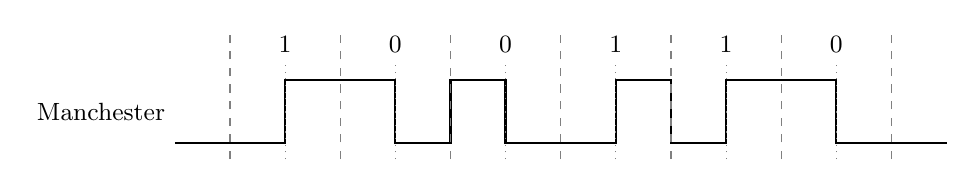
\begin{tikzpicture}[>=latex, font=\small]
  \draw[thick] (-0.7,0) -- (0.7,0) -- (0.7,0.8) -- (2.1,0.8) -- (2.1,0) -- (2.8,0) -- (2.8,0.8) -- (3.5,0.8) -- (3.5,0) -- (4.9,0) -- (4.9,0.8) -- (5.6,0.8) -- (5.6,0) -- (6.3,0) -- (6.3,0.8) -- (7.7,0.8) -- (7.7,0) -- (9.1,0);
  \foreach \i in {0,...,6} \draw[gray, dashed] (1.4*\i,-0.2) -- (1.4*\i,1.4);
  \foreach \i in {0,...,5} \draw[gray, dotted] (1.4*\i+0.7,-0.2) -- (1.4*\i+0.7,1.0);
  \foreach \i/\b in {0/1,1/0,2/0,3/1,4/1,5/0} \node at (1.4*\i+0.7,1.25) {\b};
  \node[left] at (-0.7,0.4) {Manchester};
\end{tikzpicture}
\end{center}

\subsubsection{CRCs: a little algebra that pays off}\label{sec:crc}

Several protocols end with a CRC (USB CRC-5 and CRC-16, CAN CRC-15,
Ethernet CRC-32, and many I2C/SPI sensors use CRC-8). Doing CRCs in
software on an emulator costs many instructions per bit. A small
programmable CRC unit makes them free, and the mathematics shows that one
unit covers them all.

\begin{definition}[CRC]
Treat a bit string $m_{n-1}\dots m_0$ as the polynomial
$M(x)=\sum_i m_i x^i$ over the field $\mathbb{F}_2=\{0,1\}$, where addition
is XOR. Fix a \emph{generator} $G(x)$ of degree $r$. The CRC of $M$ is the
remainder $R(x) = M(x)\,x^r \bmod G(x)$, a polynomial of degree $<r$,
i.e.\ $r$ bits.
\end{definition}

\begin{theorem}\label{thm:crc}
The transmitted codeword $T(x) = M(x)x^r + R(x)$ is divisible by $G(x)$.
Consequently the receiver can check a message by testing whether the
received polynomial is divisible by $G$. Every error pattern $E(x)$ with
$G \nmid E$ is detected. If $G$ has a nonzero constant term and degree
$r$, every burst error of length at most $r$ is detected.
\end{theorem}
\begin{proof}
By the division algorithm, $M x^r = Q G + R$. In characteristic 2,
subtraction equals addition, so $T = Mx^r + R = QG$. A received word
$T+E$ is divisible by $G$ iff $G\mid E$, so the errors that go undetected
are exactly those with $G \mid E$. A burst of length $b\le r$ has the form
$E = x^j B(x)$ with $\deg B = b-1 < r$ and $B(0)=1$. Since $G(0)=1$, $x$
does not divide $G$, so $\gcd(G, x^j) = 1$. If $G \mid x^jB$ then
$G\mid B$, which is impossible: $B\neq0$ and $\deg B<\deg G$.
\end{proof}

\begin{proposition}[Bit-serial LFSR]\label{prop:lfsr}
Let $g$ be the $r$-bit vector of the coefficients of $G$ below $x^r$. Keep an
$r$-bit state $s$ (bit $r-1$ is the coefficient of $x^{r-1}$), starting at
0. For each message bit $b$, from $m_{n-1}$ down to $m_0$, update
\[
  f = s_{r-1}\oplus b, \qquad s \gets (s \ll 1)\ \oplus\ (f\cdot g).
\]
After the last bit, $s = M(x)x^r \bmod G(x)$.
\end{proposition}
\begin{proof}
Let $M_k$ be the polynomial of the first $k$ message bits, so that
$M_{k+1} = x M_k + b$. Claim: after $k$ bits, $s = M_k x^r \bmod G$. This
holds for $k=0$. Step: we need $(xM_k + b)x^r \bmod G
= (x\cdot s + b\,x^r) \bmod G$. The polynomial $x\cdot s + bx^r$ has degree
at most $r$, with $x^r$ coefficient $s_{r-1}\oplus b = f$. Reducing it once
modulo $G$ removes that term by adding $f\cdot G$. That leaves
$(s\ll1)\oplus f\cdot g$ in the low $r$ bits, which is the update rule.
\end{proof}

This is a shift register with XOR gates at the positions where $g$ has a 1,
a \emph{linear feedback shift register}. Here is the USB CRC-5,
$G = x^5+x^2+1$ ($g = 00101_2$):
\begin{center}
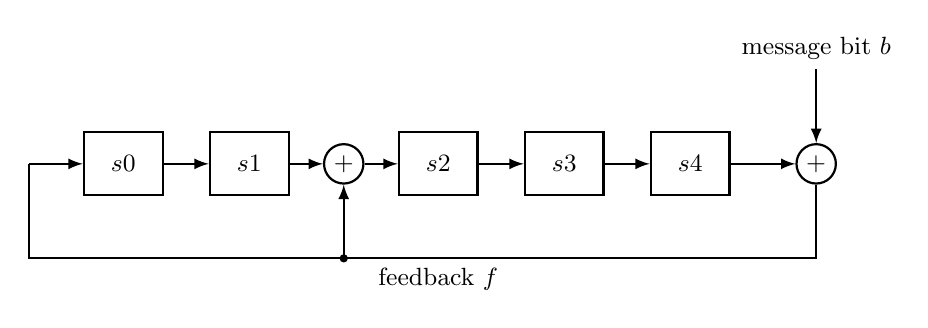
\begin{tikzpicture}[>=latex, thick, font=\small]
  \foreach \n/\x in {s0/1, s1/2.6, s2/5.0, s3/6.6, s4/8.2}
    \node[draw, minimum width=1cm, minimum height=0.8cm] (\n) at (\x,0) {$\n$};
  \node[circle, draw, inner sep=0pt, minimum size=0.5cm] (x2) at (3.8,0) {$+$};
  \node[circle, draw, inner sep=0pt, minimum size=0.5cm] (xi) at (9.8,0) {$+$};
  \draw[->] (s0) -- (s1);
  \draw[->] (s1) -- (x2);
  \draw[->] (x2) -- (s2);
  \draw[->] (s2) -- (s3);
  \draw[->] (s3) -- (s4);
  \draw[->] (s4) -- (xi);
  \draw[->] (9.8,1.2) node[above]{message bit $b$} -- (xi);
  \draw (xi.south) -- (9.8,-1.2) -- (-0.2,-1.2) -- (-0.2,0);
  \draw[->] (-0.2,0) -- (s0);
  \draw[->] (3.8,-1.2) -- (x2);
  \fill (3.8,-1.2) circle (1.5pt);
  \node[below] at (5,-1.2) {feedback $f$};
\end{tikzpicture}
\end{center}

Real CRC standards add three parameters to the pure remainder: an initial
register value, whether bits are reflected (fed LSB first), and a final
XOR. This is the ``Rocksoft model'' from Ross Williams' \emph{A Painless
Guide to CRC Error Detection Algorithms}. If the polynomial and seed are
registers rather than constants, one unit handles every standard:
{\small
\begin{verbatim}
`default_nettype none
// Bit-serial CRC with a run-time programmable generator polynomial.
// poly holds G(x) without its x^W term, e.g. 32'h04C11DB7 for CRC-32.
module crc_serial #(parameter W = 32) (
    input  wire         clk,
    input  wire         init,        // load seed (synchronous)
    input  wire [W-1:0] seed,
    input  wire [W-1:0] poly,
    input  wire         bit_valid,
    input  wire         bit_in,      // message bits in transmission order
    output reg  [W-1:0] crc
);
  wire fb = crc[W-1] ^ bit_in;
  always @(posedge clk)
    if (init)           crc <= seed;
    else if (bit_valid) crc <= {crc[W-2:0], 1'b0} ^ (fb ? poly : {W{1'b0}});
endmodule
\end{verbatim}
}
I tested this 32-bit instance against the standard check values (the CRC of
the ASCII string \texttt{"123456789"}). It reproduces CRC-32/Ethernet
(\texttt{0xCBF43926}), CRC-16/USB (\texttt{0xB4C8}) and CRC-5/USB
(\texttt{0x19}). The bytes were fed LSB first, as on the wire. A $w$-bit CRC
runs in the top $w$ bits by setting \texttt{poly = g << (32-w)} and
\texttt{seed = init << (32-w)}; the result is then reflected and XORed as
the standard specifies. In other words: \emph{one 32-bit register, a few
dozen gates, and every CRC in this lesson.} That is the kind of general
primitive the judges' flexibility criterion rewards.

\subsubsection{Summary: what an architecture must provide}
\begin{table}[ht]
\centering
\small
\begin{tabular}{|p{2.1cm}|p{3.0cm}|p{3.2cm}|p{5.6cm}|}
\hline
Protocol & Pins & Who owns timing & Demands \\ \hline
UART & TX out, RX in & each side, own baud & baud divider; RX: wait for edge,
  sample mid-bit; bit counting \\ \hline
SPI ctrl. & SCK, MOSI, CS out; MISO in & you & two pin updates per bit;
  4 modes; word size; MSB/LSB first \\ \hline
SPI target & SCK, MOSI, CS in; MISO out & external SCK & edge detection;
  low latency to MISO \\ \hline
I2C & 2 open-drain & you (controller), but stretchable & per-cycle output
  enable; wait for pin level; START/STOP detection (target) \\ \hline
JTAG & 3 out, 1 in & you & long shifts; scripted TMS sequences \\ \hline
SWD & clock out, 1 bidir & you & direction change on exact cycles; parity
  \\ \hline
PS/2 & 2 open-drain & device's clock & follow an external clock; parity \\
  \hline
CAN & TX out, RX in (transceiver) & bus, with resync & read-back each bit;
  bit stuffing; CRC-15; edge resync \\ \hline
USB LS & D+, D$-$ bidir & 1.5\,Mb/s, recovered & NRZI; (de)stuffing; SE0;
  CRC-5/16; fast turnaround \\ \hline
10BASE-T & diff.\ out, analogue in & 10\,Mb/s, recovered & Manchester at
  20\,MHz transitions; CRC-32; link pulses \\ \hline
\end{tabular}
\caption{What each protocol asks of the hardware.}\label{tab:needs}
\end{table}

The common core is small: \emph{shift bits in and out, count, wait for a pin
condition or a time, drive pins and pin directions on exact cycles, and
exchange words with the host}. On top of that sit optional accelerators:
CRC, stuffing, NRZI/Manchester, edge-tracking clock recovery. A PIO is
precisely the first list done extremely well. The second list is where you
can go further than the PIO.

% ---------------------------------------------------------------------------
\subsection{How the RP2040 PIO is built}\label{sec:pio}

\paragraph{Motivation.} The PIO is the reference point the judges named, and
you already know how to program it. Knowing how it is built tells you which
of its features are nearly free in hardware and which are expensive. That
is what you need to know to design something better within 32 tiles.

\paragraph{A note on sources.} Raspberry Pi documents the PIO's
programmer-visible behaviour precisely, in chapter~3 of the RP2040 datasheet,
but has not published its RTL. Below, \textbf{(D)} marks documented behaviour
and \textbf{(R)} marks my reconstruction: one way to build hardware that
matches every documented behaviour, not necessarily the way Raspberry Pi
built it. Open-source Verilog re-implementations exist (for example Lawrie
Griffiths' \texttt{fpga\_pio}). They are worth reading once you have your own
picture.

\subsubsection{The block (D)}

An RP2040 has two PIO blocks; an RP2350 has three. Each block contains four
state machines (SMs), one 32-instruction memory of 16-bit words shared by
all four, eight IRQ flags shared by all four, and access to every GPIO.
Each SM has a 4-word TX FIFO (system $\to$ SM) and a 4-word RX FIFO
(SM $\to$ system) of 32-bit words. The two can be joined into one 8-word
FIFO in one direction. The system writes instructions through the bus. The
instruction memory is \emph{write-only} from the bus (registers
\texttt{INSTR\_MEM0}--\texttt{INSTR\_MEM31}).

\begin{center}
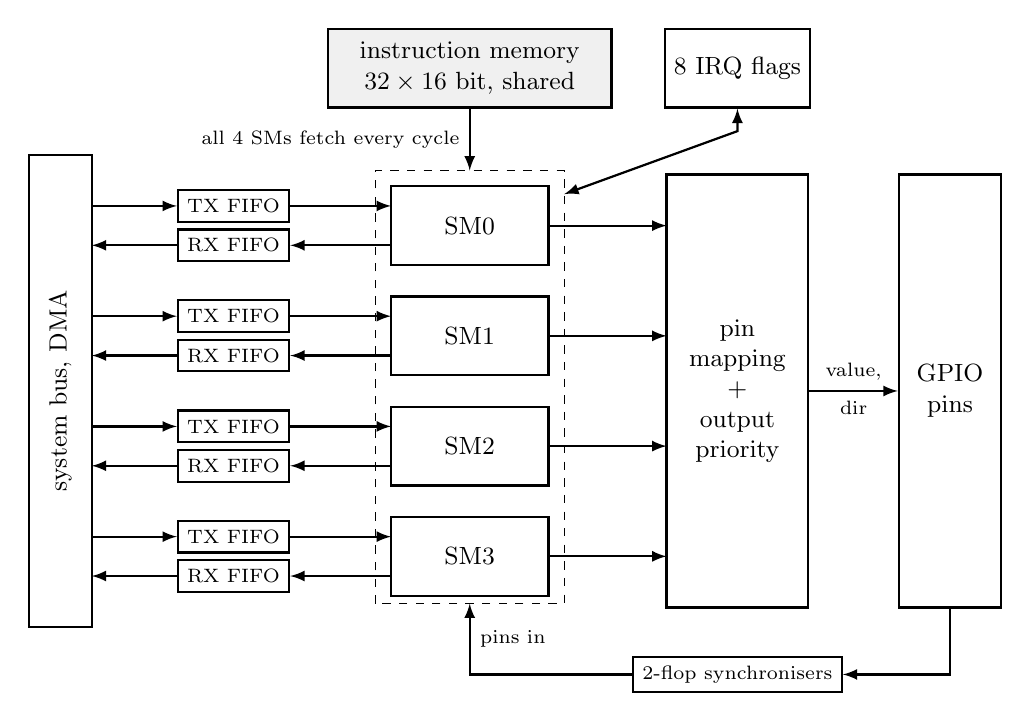
\begin{tikzpicture}[>=latex, font=\small, thick,
    box/.style={draw, align=center, minimum height=1.0cm}]
  \node[draw, minimum width=0.8cm, minimum height=6.0cm] (bus) at (0,2.7) {};
  \node[rotate=90] at (0,2.7) {system bus, DMA};
  \node[box, minimum width=3.6cm, fill=gray!12] (imem) at (5.2,6.8)
    {instruction memory\\$32\times16$ bit, shared};
  \node[box, minimum width=1.8cm] (irq) at (8.6,6.8) {8 IRQ flags};
  \draw[dashed, thin] (4.0,0.0) rectangle (6.4,5.5);
  \foreach \i/\y in {0/4.8,1/3.4,2/2.0,3/0.6} {
    \node[box, minimum width=2.0cm] (sm\i) at (5.2,\y) {SM\i};
    \node[draw, font=\scriptsize, minimum width=1.4cm, minimum height=0.35cm]
      (tx\i) at (2.2,\y+0.25) {TX FIFO};
    \node[draw, font=\scriptsize, minimum width=1.4cm, minimum height=0.35cm]
      (rx\i) at (2.2,\y-0.25) {RX FIFO};
    \draw[->] (0.4,\y+0.25) -- (tx\i.west);
    \draw[->] (tx\i.east) -- (4.2,\y+0.25);
    \draw[->] (4.2,\y-0.25) -- (rx\i.east);
    \draw[->] (rx\i.west) -- (0.4,\y-0.25);
    \draw[->] (6.2,\y) -- (7.7,\y);
  }
  \draw[->] (imem.south) -- node[left, font=\scriptsize]
    {all 4 SMs fetch every cycle} (5.2,5.5);
  \draw[<->] (irq.south) -- (8.6,6.0) -- (6.4,5.2);
  \node[box, minimum width=1.8cm, minimum height=5.5cm] (map) at (8.6,2.7)
    {pin\\mapping\\+\\output\\priority};
  \node[box, minimum width=1.3cm, minimum height=5.5cm] (gpio) at (11.3,2.7)
    {GPIO\\pins};
  \draw[->] (map.east) -- node[above, font=\scriptsize]{value,} node[below,
    font=\scriptsize]{dir} (gpio.west);
  \node[draw, font=\scriptsize] (sync) at (8.6,-0.9) {2-flop synchronisers};
  \draw[->] (gpio.south) -- (11.3,-0.9) -- (sync.east);
  \draw[->] (sync.west) -- (5.2,-0.9) -- node[right, font=\scriptsize]
    {pins in} (5.2,0.0);
\end{tikzpicture}
\end{center}

\subsubsection{One state machine's state (D)}
\begin{center}
\begin{tabular}{|l|l|}
\hline
\texttt{PC} & 5 bits \\
\texttt{X}, \texttt{Y} & 32-bit scratch registers \\
\texttt{OSR} + shift count & 32-bit output shift register, count 0--32 \\
\texttt{ISR} + shift count & 32-bit input shift register, count 0--32 \\
delay counter & up to 31 idle cycles after an instruction \\
clock divider & 16-bit integer + 8-bit fraction \\
\texttt{EXECCTRL} & wrap top/bottom, side-set enable/pindir mode, JMP pin,
  status select \\
\texttt{SHIFTCTRL} & shift directions, autopush/autopull, thresholds, FIFO
  join \\
\texttt{PINCTRL} & base pin and count for OUT, SET, side-set; base for IN
  \\ \hline
\end{tabular}
\end{center}

\subsubsection{Instruction encoding (D)}
Every instruction is 16 bits: a 3-bit opcode, a 5-bit field shared between
delay and side-set, and 8 operand bits. With $n$ side-set bits configured
(plus one more if side-set is optional, as an enable flag), $5-n$ bits remain
for the delay.
\begin{center}
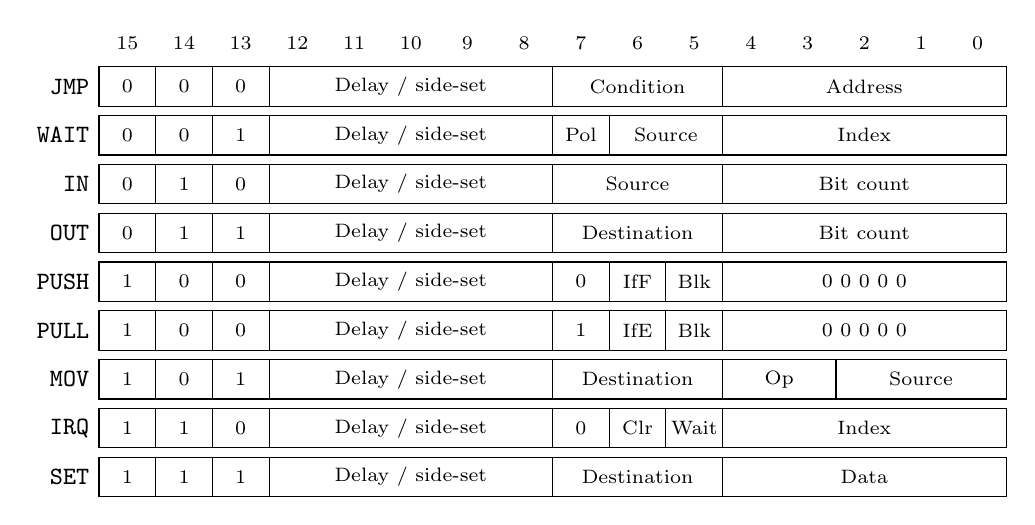
\begin{tikzpicture}[font=\scriptsize]
  \node at (11.16,0.3) {0};
  \node at (10.44,0.3) {1};
  \node at (9.72,0.3) {2};
  \node at (9,0.3) {3};
  \node at (8.28,0.3) {4};
  \node at (7.56,0.3) {5};
  \node at (6.84,0.3) {6};
  \node at (6.12,0.3) {7};
  \node at (5.4,0.3) {8};
  \node at (4.68,0.3) {9};
  \node at (3.96,0.3) {10};
  \node at (3.24,0.3) {11};
  \node at (2.52,0.3) {12};
  \node at (1.8,0.3) {13};
  \node at (1.08,0.3) {14};
  \node at (0.36,0.3) {15};
  \node[left, font=\small\ttfamily] at (0,-0.25) {JMP};
  \draw (0,0) rectangle (0.72,-0.5); \node at (0.36,-0.25) {0};
  \draw (0.72,0) rectangle (1.44,-0.5); \node at (1.08,-0.25) {0};
  \draw (1.44,0) rectangle (2.16,-0.5); \node at (1.8,-0.25) {0};
  \draw (2.16,0) rectangle (5.76,-0.5); \node at (3.96,-0.25) {Delay / side-set};
  \draw (5.76,0) rectangle (7.92,-0.5); \node at (6.84,-0.25) {Condition};
  \draw (7.92,0) rectangle (11.52,-0.5); \node at (9.72,-0.25) {Address};
  \node[left, font=\small\ttfamily] at (0,-0.87) {WAIT};
  \draw (0,-0.62) rectangle (0.72,-1.12); \node at (0.36,-0.87) {0};
  \draw (0.72,-0.62) rectangle (1.44,-1.12); \node at (1.08,-0.87) {0};
  \draw (1.44,-0.62) rectangle (2.16,-1.12); \node at (1.8,-0.87) {1};
  \draw (2.16,-0.62) rectangle (5.76,-1.12); \node at (3.96,-0.87) {Delay / side-set};
  \draw (5.76,-0.62) rectangle (6.48,-1.12); \node at (6.12,-0.87) {Pol};
  \draw (6.48,-0.62) rectangle (7.92,-1.12); \node at (7.2,-0.87) {Source};
  \draw (7.92,-0.62) rectangle (11.52,-1.12); \node at (9.72,-0.87) {Index};
  \node[left, font=\small\ttfamily] at (0,-1.49) {IN};
  \draw (0,-1.24) rectangle (0.72,-1.74); \node at (0.36,-1.49) {0};
  \draw (0.72,-1.24) rectangle (1.44,-1.74); \node at (1.08,-1.49) {1};
  \draw (1.44,-1.24) rectangle (2.16,-1.74); \node at (1.8,-1.49) {0};
  \draw (2.16,-1.24) rectangle (5.76,-1.74); \node at (3.96,-1.49) {Delay / side-set};
  \draw (5.76,-1.24) rectangle (7.92,-1.74); \node at (6.84,-1.49) {Source};
  \draw (7.92,-1.24) rectangle (11.52,-1.74); \node at (9.72,-1.49) {Bit count};
  \node[left, font=\small\ttfamily] at (0,-2.11) {OUT};
  \draw (0,-1.86) rectangle (0.72,-2.36); \node at (0.36,-2.11) {0};
  \draw (0.72,-1.86) rectangle (1.44,-2.36); \node at (1.08,-2.11) {1};
  \draw (1.44,-1.86) rectangle (2.16,-2.36); \node at (1.8,-2.11) {1};
  \draw (2.16,-1.86) rectangle (5.76,-2.36); \node at (3.96,-2.11) {Delay / side-set};
  \draw (5.76,-1.86) rectangle (7.92,-2.36); \node at (6.84,-2.11) {Destination};
  \draw (7.92,-1.86) rectangle (11.52,-2.36); \node at (9.72,-2.11) {Bit count};
  \node[left, font=\small\ttfamily] at (0,-2.73) {PUSH};
  \draw (0,-2.48) rectangle (0.72,-2.98); \node at (0.36,-2.73) {1};
  \draw (0.72,-2.48) rectangle (1.44,-2.98); \node at (1.08,-2.73) {0};
  \draw (1.44,-2.48) rectangle (2.16,-2.98); \node at (1.8,-2.73) {0};
  \draw (2.16,-2.48) rectangle (5.76,-2.98); \node at (3.96,-2.73) {Delay / side-set};
  \draw (5.76,-2.48) rectangle (6.48,-2.98); \node at (6.12,-2.73) {0};
  \draw (6.48,-2.48) rectangle (7.2,-2.98); \node at (6.84,-2.73) {IfF};
  \draw (7.2,-2.48) rectangle (7.92,-2.98); \node at (7.56,-2.73) {Blk};
  \draw (7.92,-2.48) rectangle (11.52,-2.98); \node at (9.72,-2.73) {0 0 0 0 0};
  \node[left, font=\small\ttfamily] at (0,-3.35) {PULL};
  \draw (0,-3.1) rectangle (0.72,-3.6); \node at (0.36,-3.35) {1};
  \draw (0.72,-3.1) rectangle (1.44,-3.6); \node at (1.08,-3.35) {0};
  \draw (1.44,-3.1) rectangle (2.16,-3.6); \node at (1.8,-3.35) {0};
  \draw (2.16,-3.1) rectangle (5.76,-3.6); \node at (3.96,-3.35) {Delay / side-set};
  \draw (5.76,-3.1) rectangle (6.48,-3.6); \node at (6.12,-3.35) {1};
  \draw (6.48,-3.1) rectangle (7.2,-3.6); \node at (6.84,-3.35) {IfE};
  \draw (7.2,-3.1) rectangle (7.92,-3.6); \node at (7.56,-3.35) {Blk};
  \draw (7.92,-3.1) rectangle (11.52,-3.6); \node at (9.72,-3.35) {0 0 0 0 0};
  \node[left, font=\small\ttfamily] at (0,-3.97) {MOV};
  \draw (0,-3.72) rectangle (0.72,-4.22); \node at (0.36,-3.97) {1};
  \draw (0.72,-3.72) rectangle (1.44,-4.22); \node at (1.08,-3.97) {0};
  \draw (1.44,-3.72) rectangle (2.16,-4.22); \node at (1.8,-3.97) {1};
  \draw (2.16,-3.72) rectangle (5.76,-4.22); \node at (3.96,-3.97) {Delay / side-set};
  \draw (5.76,-3.72) rectangle (7.92,-4.22); \node at (6.84,-3.97) {Destination};
  \draw (7.92,-3.72) rectangle (9.36,-4.22); \node at (8.64,-3.97) {Op};
  \draw (9.36,-3.72) rectangle (11.52,-4.22); \node at (10.44,-3.97) {Source};
  \node[left, font=\small\ttfamily] at (0,-4.59) {IRQ};
  \draw (0,-4.34) rectangle (0.72,-4.84); \node at (0.36,-4.59) {1};
  \draw (0.72,-4.34) rectangle (1.44,-4.84); \node at (1.08,-4.59) {1};
  \draw (1.44,-4.34) rectangle (2.16,-4.84); \node at (1.8,-4.59) {0};
  \draw (2.16,-4.34) rectangle (5.76,-4.84); \node at (3.96,-4.59) {Delay / side-set};
  \draw (5.76,-4.34) rectangle (6.48,-4.84); \node at (6.12,-4.59) {0};
  \draw (6.48,-4.34) rectangle (7.2,-4.84); \node at (6.84,-4.59) {Clr};
  \draw (7.2,-4.34) rectangle (7.92,-4.84); \node at (7.56,-4.59) {Wait};
  \draw (7.92,-4.34) rectangle (11.52,-4.84); \node at (9.72,-4.59) {Index};
  \node[left, font=\small\ttfamily] at (0,-5.21) {SET};
  \draw (0,-4.96) rectangle (0.72,-5.46); \node at (0.36,-5.21) {1};
  \draw (0.72,-4.96) rectangle (1.44,-5.46); \node at (1.08,-5.21) {1};
  \draw (1.44,-4.96) rectangle (2.16,-5.46); \node at (1.8,-5.21) {1};
  \draw (2.16,-4.96) rectangle (5.76,-5.46); \node at (3.96,-5.21) {Delay / side-set};
  \draw (5.76,-4.96) rectangle (7.92,-5.46); \node at (6.84,-5.21) {Destination};
  \draw (7.92,-4.96) rectangle (11.52,-5.46); \node at (9.72,-5.21) {Data};
\end{tikzpicture}
\end{center}
Field values on the RP2040: JMP conditions are
\texttt{always}, \texttt{!X}, \texttt{X-{}-}, \texttt{!Y}, \texttt{Y-{}-},
\texttt{X!=Y}, \texttt{PIN}, \texttt{!OSRE}. IN sources are PINS, X, Y, NULL,
ISR, OSR. OUT destinations are PINS, X, Y, NULL, PINDIRS, PC, ISR, EXEC. MOV
sources are PINS, X, Y, NULL, STATUS, ISR, OSR, with an op of none, invert or
bit-reverse. SET destinations are PINS, X, Y, PINDIRS. A bit count of 0 means
32. The RP2350's PIO (``version 1'') adds a few encodings on top.

\subsubsection{Execution semantics (D)}
These are the rules your own design will compete with:
\begin{enumerate}[label=\arabic*.]
  \item \textbf{One instruction per (enabled) cycle.} Every instruction,
    including a taken JMP, takes exactly one cycle unless it stalls. Then
    come its delay cycles, during which the SM does nothing.
  \item \textbf{Stalls.} WAIT on an unmet condition, a blocking PULL with an
    empty TX FIFO, a blocking PUSH with a full RX FIFO, autopull/autopush that
    cannot complete, and \texttt{IRQ wait} all hold the SM at the same
    instruction. Delay cycles begin only once the stall ends.
  \item \textbf{Side-set} happens when the instruction issues, \emph{even if
    it stalls}. That is how \texttt{spi\_cpha0} parks SCK low while waiting
    for data. Within one SM, side-set takes priority over OUT/SET writes to
    the same pin.
  \item \textbf{Wrap.} After executing the instruction at \texttt{wrap\_top},
    the PC continues at \texttt{wrap\_bottom}, unless the instruction
    jumped. So a loop costs no instruction.
  \item \textbf{\texttt{JMP X-{}-}} jumps if X is nonzero \emph{before} the
    decrement, and decrements either way. \texttt{set x, 7} followed by a
    \texttt{jmp x-{}-} loop runs 8 times.
  \item \textbf{Shift registers.} \texttt{OUT dst, n} shifts $n$ bits out of
    the OSR (left or right, as configured) and increments its shift count.
    \texttt{IN src, n} shifts $n$ bits into the ISR. With \emph{autopull},
    the OSR refills from the TX FIFO when its count reaches the threshold,
    stalling if the FIFO is empty. With \emph{autopush}, the ISR goes to the
    RX FIFO when its count reaches the threshold. This keeps loops like SPI
    at 2 instructions per bit, with no explicit PULL/PUSH.
  \item \textbf{Pins.} OUT, SET and side-set each write a contiguous group
    of pins starting at a configured base (wrapping modulo 32). IN reads 32
    bits starting at its base. If two SMs write the same pin in the same
    cycle, the highest-numbered SM wins.
  \item \textbf{Inputs are synchronised} by two flops per GPIO (bypassable),
    which costs two cycles of latency (\cref{sec:meta}).
  \item \textbf{Clock divider.} The SM runs on the system clock but executes
    only on cycles selected by a 16.8 fractional divider. The fractional
    part produces one system clock of jitter.
  \item \textbf{EXEC.} \texttt{OUT EXEC} and \texttt{MOV EXEC} execute a data
    word as the next instruction, and the system can also force an
    instruction into an SM. Programs can therefore generate instructions.
  \item \textbf{IRQ flags} let SMs synchronise with each other (one sets
    a flag, another WAITs on it) and interrupt the CPU.
\end{enumerate}

\subsubsection{A cycle-by-cycle trace}
The \texttt{uart\_tx} program from \texttt{pico-examples}, with OUT and
side-set mapped to the same pin and the divider set so that 8 SM cycles make
one bit:
\begin{verbatim}
.program uart_tx
.side_set 1 opt
    pull       side 1 [7]  ; Assert stop bit, or stall with line in idle state
    set x, 7   side 0 [7]  ; Preload bit counter, assert start bit for 8 clocks
bitloop:                   ; This loop will run 8 times (8n1 UART)
    out pins, 1            ; Shift 1 bit from OSR to the first OUT pin
    jmp x-- bitloop   [6]  ; Each loop iteration is 8 cycles.
\end{verbatim}
\begin{center}
\small
\begin{tabular}{|r|c|l|l|c|}
\hline
SM cycle & PC & executing & effect & TX \\ \hline
0 & 0 & \texttt{pull side 1 [7]} & OSR $\gets$ byte (stalls here if FIFO
  empty) & 1 \\
1--7 & 0 & delay & --- & 1 \\
8 & 1 & \texttt{set x, 7 side 0 [7]} & X $\gets$ 7 & 0 (start) \\
9--15 & 1 & delay & --- & 0 \\
16 & 2 & \texttt{out pins, 1} & pin $\gets$ OSR[0], OSR $\gg$= 1 & D0 \\
17 & 3 & \texttt{jmp x-{}- bitloop [6]} & X$=7\neq0$: jump; X $\gets$ 6 & D0 \\
18--23 & 3 & delay & --- & D0 \\
24--31 & 2, 3 & same, X: $6\to5$ & & D1 \\
\multicolumn{5}{|c|}{\ldots} \\
72 & 2 & \texttt{out pins, 1} & & D7 \\
73 & 3 & \texttt{jmp x-{}- bitloop [6]} & X$=0$: fall through;
  X $\gets$ \texttt{0xFFFFFFFF} & D7 \\
74--79 & 3 & delay & --- & D7 \\
80 & 0 & \texttt{pull side 1 [7]} & wrap to 0; stop bit begins & 1 \\ \hline
\end{tabular}
\end{center}
Every bit lasts exactly 8 cycles, because the cycle counts were designed
that way: 1 + 7 for the start bit, (1) + (1 + 6) for each data bit, and
1 + 7 for the stop bit. There is no explicit jump back to the start: the
implicit \texttt{.wrap} at the end of the program makes the loop free.

\subsubsection{Microarchitecture (R)}
A plausible implementation of one SM, consistent with all of the above:

\begin{center}
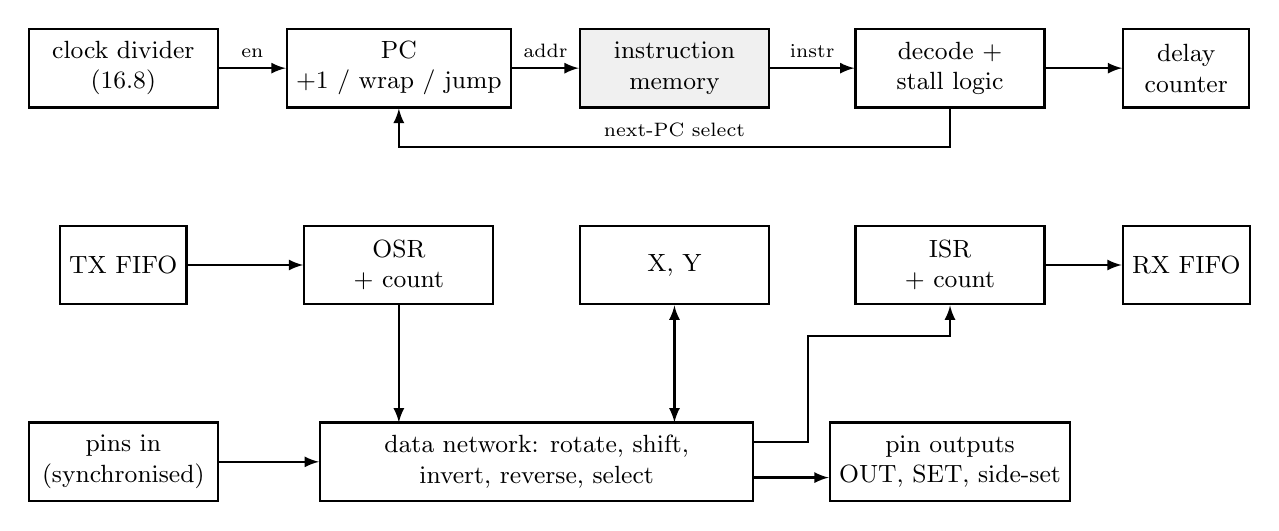
\begin{tikzpicture}[>=latex, font=\small, thick,
    box/.style={draw, align=center, minimum width=2.4cm, minimum height=1.0cm}]
  \node[box] (div) at (0.4,5) {clock divider\\(16.8)};
  \node[box] (pc) at (3.9,5) {PC\\$+1$ / wrap / jump};
  \node[box, fill=gray!12] (im) at (7.4,5) {instruction\\memory};
  \node[box] (dec) at (10.9,5) {decode +\\stall logic};
  \node[box, minimum width=1.6cm] (dly) at (13.9,5) {delay\\counter};
  \node[box, minimum width=1.6cm] (txf) at (0.4,2.5) {TX FIFO};
  \node[box] (osr) at (3.9,2.5) {OSR\\+ count};
  \node[box] (xy) at (7.4,2.5) {X, Y};
  \node[box] (isr) at (10.9,2.5) {ISR\\+ count};
  \node[box, minimum width=1.6cm] (rxf) at (13.9,2.5) {RX FIFO};
  \node[box, minimum width=2.4cm] (pin) at (0.4,0) {pins in\\(synchronised)};
  \node[box, minimum width=5.5cm] (mux) at (5.65,0)
    {data network: rotate, shift,\\invert, reverse, select};
  \node[box] (pout) at (10.9,0) {pin outputs\\OUT, SET, side-set};
  \draw[->] (div) -- node[above, font=\scriptsize]{en} (pc);
  \draw[->] (pc) -- node[above, font=\scriptsize]{addr} (im);
  \draw[->] (im) -- node[above, font=\scriptsize]{instr} (dec);
  \draw[->] (dec) -- (dly);
  \draw[->] (dec.south) -- (10.9,4.0) -- node[above, font=\scriptsize]
    {next-PC select} (3.9,4.0) -- (pc.south);
  \draw[->] (txf) -- (osr);
  \draw[->] (osr.south) -- (3.9,0.5);
  \draw[<->] (xy.south) -- (7.4,0.5);
  \draw[->] (8.4,0.25) -- (9.1,0.25) -- (9.1,1.6) -- (10.9,1.6) -- (isr.south);
  \draw[->] (isr) -- (rxf);
  \draw[->] (pin) -- (mux);
  \draw[->] (8.4,-0.2) -- (pout.west |- 0,-0.2);
\end{tikzpicture}
\end{center}

\begin{itemize}
  \item \textbf{No pipeline.} The instruction memory is (almost certainly)
    flip-flops with a combinational read, so the word at \texttt{PC} is
    available within the same cycle. Fetch, decode and execute all happen
    in one cycle of combinational logic, and the clock edge commits the
    result. That is why a taken JMP costs nothing extra. The price: all
    four SMs read the memory every cycle, so it needs \emph{four read
    ports}, which means four 32-to-1 multiplexers of 16 bits each.
  \item \textbf{Clock divider as an enable.} All state updates are gated by
    \texttt{en}, a pulse train from a fractional accumulator (code below).
    Nothing runs on a derived clock (\cref{sec:timing}).
  \item \textbf{Stall is one wire.} Decode produces a single \texttt{stall}
    signal from the stall conditions. When it is high, the PC, delay
    counter and data registers keep their values, but the side-set write
    still happens. That is a one-line difference in the RTL.
  \item \textbf{Next PC} is a small priority mux: jump target if jumping,
    \texttt{wrap\_bottom} if \texttt{PC == wrap\_top}, otherwise
    $\texttt{PC}+1$. Wrap is one 5-bit comparator, which is why it is free.
  \item \textbf{Shifters.} Shifting by 1--32 bits in a single cycle needs a
    barrel shifter: $\log_2 32 = 5$ levels of 2-to-1 multiplexers, about
    160 gates for 32 bits (measured below). Pin groups at a configurable
    base are a \emph{rotation} of the 32-bit pin vector, the same structure
    again.
  \item \textbf{Pin outputs.} Each SM produces, per pin, a value, a
    value-write-enable, a direction and a direction-write-enable. The block
    merges the four SMs with a fixed priority, and per-pin registers drive
    the GPIO mux.
  \item \textbf{FIFOs without clock crossing.} The SMs run on the
    \emph{system} clock, the same clock as the bus. So the FIFOs are simple
    synchronous FIFOs, with no asynchronous clock-crossing logic. Keep this
    property in your design: one clock everywhere.
\end{itemize}

\paragraph{The fractional divider.} This accumulator generates the enable:
{\small
\begin{verbatim}
`default_nettype none
// Fractional clock-enable generator: one-cycle pulse on `en`, on average
// once every (div_int + div_frac/256) clocks. div_int must be >= 1.
module clkdiv (
    input  wire        clk,
    input  wire        rst_n,
    input  wire [15:0] div_int,
    input  wire [7:0]  div_frac,
    output reg         en
);
  wire [24:0] div  = {1'b0, div_int, div_frac};  // period in 1/256 clocks
  reg  [24:0] acc;                               // invariant: acc < div
  wire [24:0] next = acc + 25'd256;              // one clock = 256 units

  always @(posedge clk) begin
    if (!rst_n) begin
      acc <= 0;
      en  <= 1'b0;
    end else if (next >= div) begin
      acc <= next - div;
      en  <= 1'b1;
    end else begin
      acc <= next;
      en  <= 1'b0;
    end
  end
endmodule
\end{verbatim}
}
\begin{proposition}\label{prop:clkdiv}
Let $D = \texttt{div}/256 \ge 1$ be the divisor in clock cycles. After reset,
the $k$-th pulse occurs in cycle $\lceil kD\rceil$ (up to the constant
one-cycle delay of the output register). Consequently every gap between
pulses is $\lfloor D\rfloor$ or $\lceil D\rceil$, and over $N$ cycles the
number of pulses is $\lfloor N/D\rfloor$.
\end{proposition}
\begin{proof}
Let $p_t$ be the number of pulses and $a_t$ the accumulator after $t$
cycles, with $a_0=p_0=0$. Each cycle adds 256 to the accumulator and each
pulse subtracts \texttt{div}, so $256t = p_t\cdot\texttt{div} + a_t$. We
show by induction that $0\le a_t<\texttt{div}$. If it holds at $t$, then
$a_t + 256 < 2\,\texttt{div}$ because $\texttt{div}\ge256$. So at most one
subtraction is needed, and it leaves $0 \le a_{t+1} < \texttt{div}$. With
the invariant, $p_t = \lfloor 256t/\texttt{div}\rfloor = \lfloor t/D\rfloor$.
The $k$-th pulse is the first $t$ with $t/D \ge k$, i.e.\
$t=\lceil kD\rceil$. Gaps are
$\lceil (k+1)D\rceil-\lceil kD\rceil\in\{\lfloor D\rfloor,\lceil D\rceil\}$.
\end{proof}
This is Bresenham's line algorithm in disguise: it steps one clock at a time
and emits a pulse whenever the accumulated error crosses one period. With
$D=2.5$ the testbench sees gaps of exactly 2, 3, 2, 3, \ldots, 400 pulses
in 1000 cycles. I also proved the invariant $a_t<\texttt{div}$ formally
(\cref{sec:verif}).

\subsubsection{A toy PIO in 70 lines}\label{sec:toy}

To make the reconstruction concrete, here is a working, deliberately tiny
PIO-style state machine: one output pin, a 1-bit side-set, a 3-bit delay, an
8-bit OSR, and five instructions. The opcode numbers follow the PIO
(\texttt{JMP}=000, \texttt{WAIT}=001, \texttt{OUT}=011, \texttt{PULL}=100,
\texttt{SET}=111). The other fields are simplified.
{\small
\begin{verbatim}
`default_nettype none
// A toy PIO-style state machine: one output pin, one-bit side-set.
//   [15:13] opcode  [12] side-set enable  [11] side-set value
//   [10:8]  delay   [7:0] operand (meaning depends on opcode)
module toy_sm (
    input  wire        clk,
    input  wire        rst_n,
    input  wire        en,          // clock enable from clkdiv
    input  wire        imem_we,     // program loading port
    input  wire [4:0]  imem_waddr,
    input  wire [15:0] imem_wdata,
    input  wire [4:0]  wrap_top,    // after this address, continue at 0
    input  wire [7:0]  tx_data,     // one-entry "TX FIFO" from the host
    input  wire        tx_valid,
    output wire        tx_ready,
    input  wire [7:0]  pins_in,     // already synchronised
    output reg         pin_out
);
  localparam JMP = 3'd0, WAIT = 3'd1, OUT = 3'd3, PULL = 3'd4, SET = 3'd7;

  reg [15:0] imem [0:31];
  reg [4:0]  pc, x;
  reg [7:0]  osr;
  reg [2:0]  delay;

  wire [15:0] instr   = imem[pc];   // combinational read: no fetch stage
  wire [2:0]  op      = instr[15:13];
  wire        side_en = instr[12];
  wire        side_v  = instr[11];

  wire busy  = delay != 0;          // burning delay cycles
  wire stall = (op == PULL && !tx_valid) ||
               (op == WAIT && pins_in[instr[2:0]] != instr[7]);
  assign tx_ready = en && !busy && op == PULL;

  // JMP: operand[5] selects "x--" (jump if x != 0, then decrement).
  wire       take_jmp = op == JMP && (!instr[5] || x != 0);
  wire [4:0] pc_next  = take_jmp         ? instr[4:0] :
                        pc == wrap_top   ? 5'd0       : pc + 5'd1;

  always @(posedge clk)
    if (imem_we) imem[imem_waddr] <= imem_wdata;

  always @(posedge clk) begin
    if (!rst_n) begin
      pc <= 0; x <= 0; osr <= 0; delay <= 0;
      pin_out <= 1'b1;               // idle-high, so reset is not a start bit
    end else if (en) begin
      if (busy) begin
        delay <= delay - 3'd1;
      end else begin
        if (!stall) begin
          delay <= instr[10:8];
          pc    <= pc_next;
          case (op)
            JMP:  if (instr[5]) x <= x - 5'd1;
            OUT:  begin pin_out <= osr[0]; osr <= osr >> 1; end
            PULL: osr <= tx_data;
            SET:  if (instr[5]) x <= instr[4:0]; else pin_out <= instr[0];
            default: ;
          endcase
        end
        // Last nonblocking assignment wins, so side-set beats OUT/SET,
        // and it is applied even while the instruction stalls.
        if (side_en) pin_out <= side_v;
      end
    end
  end
endmodule
\end{verbatim}
}
Map it onto the semantics list. Rule 1 is the single \texttt{always} block
gated by \texttt{en}. Rule 2 is the \texttt{stall} wire, plus the delay
counter that only reloads when an instruction completes. Rule 3 is the
side-set line placed \emph{after} the \texttt{if (!stall)} block, so it runs
even when stalled and overrides OUT/SET. Rule 4 is the \texttt{wrap\_top}
comparison in \texttt{pc\_next}. Rule 5 is \texttt{take\_jmp} testing
\texttt{x} before the decrement. The UART program assembles to:
\begin{verbatim}
addr  word    meaning
 0    0x9F00  pull         side 1 [7]   (op 100, side en=1 val=1, delay 7)
 1    0xF727  set x, 7     side 0 [7]   (op 111, side en=1 val=0, delay 7)
 2    0x6000  out pins, 1               (op 011)
 3    0x0622  jmp x-- 2    [6]          (op 000, delay 6, x-- flag, addr 2)
      wrap_top = 3
\end{verbatim}
In simulation, with a divider of 3 (so 24 clocks per bit), the testbench
checked the bytes \texttt{0x55}, \texttt{0xA3}, \texttt{0x00} and
\texttt{0xFF} sent back to back. Every bit had the right value for exactly
24 clocks, and the line stayed high while PULL stalled. A second program
(\texttt{wait 1 pin 0; set pins 1; wait 0 pin 0; set pins 0}) made the
output follow an input. Before I fixed it, the first version reset
\texttt{pin\_out} to 0: the line sat low during reset and looked like a start
bit to the receiver. That is a real failure mode, and a reason pin reset
levels should be configurable.

\paragraph{What the toy lacks}, compared with a PIO SM: multi-bit OUT/IN with
shift direction and bit counts (barrel shifters), the ISR and IN, autopull
and autopush, Y, MOV and its operations, IRQs, pin mapping with base and
count, pin directions, FIFOs deeper than one entry, EXEC, and a
configurable side-set width. Each is a well-defined increment, and adding
them one at a time, each with a test, is a sensible way to grow your own
engine.

\subsubsection{Where the area goes}\label{sec:area}
I synthesised the pieces with Yosys (generic gates: AND, OR, MUX, flip-flops,
\ldots; not IHP standard cells, so treat these as relative sizes):
\begin{center}
\begin{tabular}{|l|r|p{6.4cm}|}
\hline
block & generic cells & note \\ \hline
\texttt{uart\_tx} (fixed function) & 105 & 24 flip-flops \\
\texttt{clkdiv} (16.8) & 307 & 26 flip-flops, a 25-bit add/compare/subtract \\
32-bit barrel shifter & 167 & 129 of them MUX \\
32-bit adder & 163 & \\
\texttt{toy\_sm} total & 1241 & of which 480 flip-flops + about 450 MUX are
  its instruction memory \\
$32\times16$ memory, 4 read ports & 4822 & 512 flip-flops + read logic \\
\hline
\end{tabular}
\end{center}
Lessons:
\begin{itemize}
  \item \textbf{Instruction storage dominates.} Three quarters of the toy SM
    is its 32-word memory. A PIO-style shared memory with four
    combinational read ports costs about four times a whole toy SM.
  \item \textbf{Execution logic is cheap.} Shifters, adders and decoders are
    a few hundred gates each.
  \item \textbf{Rough budget for a faithful PIO block} (my estimate, easily
    $\pm50\%$): per SM, about 480 flip-flops (X, Y, ISR, OSR, two 4-word
    FIFOs, counters, configuration) plus 1--2K gates of logic. With four
    SMs and the shared memory, that is roughly 10--15K generic cells. The
    TT rough figure is 1K cells per tile, so 32 tiles is about 32K. A full
    PIO-class block therefore fits with room to spare, and the real question
    is what to spend the rest on. Only synthesis with the real flow tells
    you the truth (\cref{sec:flow}).
  \item Flip-flops are much larger than a NAND gate (several times), so
    flip-flop-heavy blocks such as FIFOs and memories cost more silicon
    than their cell count suggests. Mux-heavy logic maps to complex IHP
    cells and costs less than the generic count suggests.
\end{itemize}

\subsubsection{The TI PRU, for contrast}
The PRU-ICSS on TI's Sitara parts (e.g.\ AM335x, as on the BeagleBone)
takes the opposite approach. It is a small \emph{general-purpose} 32-bit
load/store RISC core at 200\,MHz, where most instructions take a single
cycle, with no caches and no pipeline surprises, so timing is deterministic.
Two registers are wired to pins: writing \texttt{R30} drives outputs, and
\texttt{R31} reads inputs. It has local instruction and data RAM and is
programmed in assembly or C.
\begin{center}
\begin{tabular}{|p{3.2cm}|p{5.2cm}|p{5.2cm}|}
\hline
& PIO & PRU \\ \hline
per-bit cost & 1--2 instructions per bit, because one instruction does
  shift + pin + delay + loop & several instructions per bit (shift, mask,
  store, branch) \\
computation & almost none (no add, no compare beyond X!=Y) & full ALU,
  memory, C compiler \\
timing & cycle-exact, delays in the instruction & cycle-exact, by counting
  instructions \\
area & tiny per SM & a whole CPU plus RAM \\ \hline
\end{tabular}
\end{center}
The design space between these two is where your entry lives. One
extreme: specialised bit engines. The other: a general core.
Interesting points in between: a PIO-like engine with a few more ALU
operations, or a PIO-like engine \emph{plus} protocol accelerators such as
the CRC of \cref{sec:crc}.

% ---------------------------------------------------------------------------
\subsection{Memories, and how they shape the pipeline}\label{sec:memory}

\paragraph{Motivation.} \Cref{sec:area} showed that instruction storage
dominates area. You have three kinds of storage to choose from, and the
choice changes your microarchitecture, not just your area.

\begin{center}
\begin{tabular}{|p{2.4cm}|p{3.6cm}|p{3.6cm}|p{3.8cm}|}
\hline
& flip-flops & latches & SRAM macro \\ \hline
density & lowest & about twice flip-flops (rough) & highest \\
read & combinational, same cycle & combinational & \textbf{synchronous}:
  address captured at an edge, data valid shortly after \\
read ports & any number (each costs a mux tree) & any number & usually 1
  (check which macro configurations exist) \\
risk & none & timing analysis of latches is subtle in open flows & fixed
  sizes, a hard macro to place, needs a simulation model for RTL and GL \\
\hline
\end{tabular}
\end{center}

\paragraph{Synchronous read and the fetch problem.} With flip-flop memory,
the instruction at \texttt{PC} is available within the same cycle
(\cref{sec:pio}). An SRAM captures its address at a clock edge and delivers
data a short access time after it. There are two ways to connect it:
\begin{enumerate}[label=(\alph*)]
  \item \textbf{Address from the \texttt{PC} register.} The word for
    \texttt{PC} arrives one cycle after \texttt{PC} changes, which is a
    two-stage pipeline (fetch, execute). When a jump executes, the next
    sequential word is already fetched and must be discarded: a one-cycle
    bubble on every taken jump.
  \item \textbf{Address from \texttt{next\_pc}}, the combinational value the
    \texttt{PC} register is about to take. The SRAM then captures the
    address at the same edge at which \texttt{PC} updates, and the
    instruction appears during the cycle it executes: no bubble. The price
    is the critical path. SRAM access, then decode, stall and next-PC
    logic, then SRAM address setup must all fit in one cycle. Get the
    numbers from the macro's timing model; at 60\,MHz this may well fit.
\end{enumerate}
With (a), keep in mind that \emph{determinism} is what protocols need, not
single-cycle jumps. A jump that always takes exactly 2 cycles is fine if your
assembler and documentation account for it. A bubble whose length depends
on runtime state is not. PIO's cycle-counting style programs, like the
\texttt{[6]} in \texttt{uart\_tx}, need every instruction's cost known
statically.

\paragraph{Sharing.} A single-port SRAM serves one engine per cycle. Ways to
feed $N$ engines:
\begin{itemize}
  \item one SRAM (or flop memory) per engine: simple, but the per-macro
    overhead adds up;
  \item one wide SRAM word holding several instructions (fetch 2--4 at
    once, buffer them per engine);
  \item \textbf{time-multiplexing} (a ``barrel'' design): one shared
    pipeline serves engine 0 in cycle 0, engine 1 in cycle 1, and so on,
    round-robin. Each of $N$ engines runs at $f/N$ with perfectly regular
    timing. The CDC 6600's peripheral processors and XMOS's hardware
    threads work this way. The post's FAQ explicitly mentions ``multiple
    engines sharing a pipeline'' as an acceptable architecture. The
    trade-off: at 60\,MHz with 4 engines, each gets 15\,M instructions per
    second, which is still 10 instructions per bit at 1.5\,Mbit/s USB.
\end{itemize}
SRAM is also the natural home for any large buffer: packet buffers for USB
or Ethernet, or a capture buffer if you add a logic-analyser mode. Follow the
SRAM walkthrough linked from the post (Ken Pettit's IHP SRAM macro guide)
before you commit to a macro, and run the full flow with it early.

% ---------------------------------------------------------------------------
\subsection{From RTL to GDS: the ASIC flow}\label{sec:flow}

\paragraph{Motivation.} On an FPGA the vendor tool's output is a bitstream
you can rewrite in seconds. On an ASIC the output is \emph{GDS}: geometry
for every mask layer, which a foundry turns into silicon you cannot change.
The flow is a pipeline of compilers and checkers, and the TT template runs
it for you (through LibreLane) on every push. You still need to understand
it, to read its reports and to know what to fix.

\begin{center}
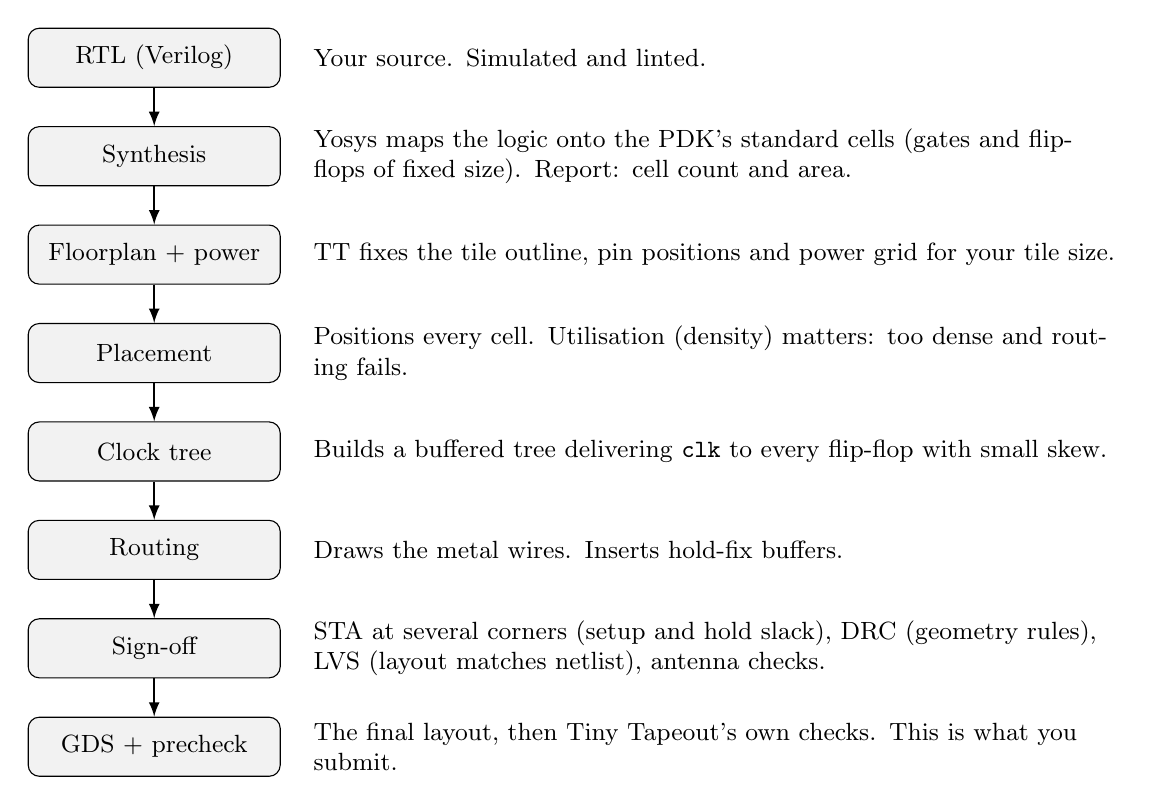
\begin{tikzpicture}[>=latex, font=\small,
    stage/.style={draw, rounded corners, minimum width=3.2cm,
      minimum height=0.75cm, align=center, fill=gray!10},
    note/.style={anchor=west, text width=10.2cm, font=\small}]
  \foreach \n/\t/\d [count=\i from 0] in {
    rtl/RTL (Verilog)/{Your source. Simulated and linted.},
    syn/Synthesis/{Yosys maps the logic onto the PDK's standard cells (gates
      and flip-flops of fixed size). Report: cell count and area.},
    fp/Floorplan + power/{TT fixes the tile outline, pin positions and power
      grid for your tile size.},
    pl/Placement/{Positions every cell. Utilisation (density) matters:
      too dense and routing fails.},
    cts/Clock tree/{Builds a buffered tree delivering \texttt{clk} to every
      flip-flop with small skew.},
    rt/Routing/{Draws the metal wires. Inserts hold-fix buffers.},
    so/Sign-off/{STA at several corners (setup and hold slack), DRC
      (geometry rules), LVS (layout matches netlist), antenna checks.},
    gds/GDS + precheck/{The final layout, then Tiny Tapeout's own checks.
      This is what you submit.}} {
    \node[stage] (\n) at (0,-1.25*\i) {\t};
    \node[note] at (1.9,-1.25*\i) {\d};
  }
  \foreach \a/\b in {rtl/syn,syn/fp,fp/pl,pl/cts,cts/rt,rt/so,so/gds}
    \draw[->, thick] (\a) -- (\b);
\end{tikzpicture}
\end{center}

\subsubsection{Standard cells and the PDK}
A \emph{PDK} (process design kit) describes a process: layer rules, device
models, and a \emph{standard-cell library} of pre-drawn gates (inverters,
NAND/NOR, AND-OR-INVERT combinations, multiplexers, flip-flops with or
without reset or enable, buffers of several drive strengths), all of the same
height so that they tile in rows. Synthesis expresses your design as a
netlist of these cells. Their area, delay and power models come from
\emph{liberty} files characterised at several corners. That is why the gate
counts in \cref{sec:area} were only relative: the real flow maps onto real
cells, some of which do the work of several generic gates.

\subsubsection{Tiny Tapeout specifics (from the template)}
\begin{itemize}
  \item \texttt{info.yaml}: \texttt{tiles} (valid values include
    \texttt{"8x4"}), \texttt{top\_module} (must start with \texttt{tt\_um\_};
    the template suggests including your GitHub username for uniqueness),
    \texttt{source\_files} (files in \texttt{src/}, each listed
    separately), \texttt{clock\_hz}, and a \texttt{pinout} section for the
    datasheet. Also edit \texttt{docs/info.md}.
  \item \texttt{test/Makefile}: update \texttt{PROJECT\_SOURCES} to match
    \texttt{source\_files}. \texttt{make -B} runs the RTL simulation (cocotb
    and Icarus by default) and writes \texttt{tb.fst}; view it with GTKWave
    or Surfer.
  \item \textbf{Gate-level simulation}: after hardening, copy
    \nolinkurl{runs/wokwi/results/final/verilog/gl/<module>.v} to
    \texttt{test/gate\_level\_netlist.v} and run \texttt{make -B GATES=yes}.
    The Makefile pulls in the CMOS5L standard-cell models
    (\texttt{PDK ?= ihp-sg13cmos5l}). The GDS GitHub Action does the copy
    for you. Run the \emph{same} cocotb tests at gate level: they then check
    the netlist, reset behaviour and synthesis/simulation mismatches.
  \item \textbf{GitHub Actions}: the template's workflows build the GDS,
    docs, tests and an FPGA bitstream. If an $8\times4$ run exceeds the
    6-hour Action limit, the post says to harden locally (TT has a
    ``local hardening'' guide) and submit through the custom-GDS action,
    which still runs precheck.
  \item \textbf{Read before you start}: TT's ``moving from FPGA to ASIC''
    page, linked from the post's FAQ.
\end{itemize}

\subsubsection{What to read in the reports}
Exact file names vary between flow versions, so search the run directory.
After every serious change, look at:
\begin{itemize}
  \item \textbf{Synthesis}: total cell count and area. Which module is
    biggest? Any unexpected latches, multiple drivers, or logic optimised
    away (a sign that something is unconnected)?
  \item \textbf{Timing}: worst setup slack and worst hold slack, over all
    corners, at your \texttt{clock\_hz}. Negative setup slack means a path
    is too long (\cref{thm:timing}); find it in the STA path report, which
    lists every cell on the path with its delay.
  \item \textbf{Design-rule violations}: max transition, max capacitance,
    max fanout, DRC, LVS, antenna. All should be zero.
  \item \textbf{Utilisation}: how full your tiles are. Routing needs space;
    a design that synthesises to 95\% of the area will not route.
\end{itemize}
Per the post: run synthesis early, check the mapped cell area, leave room
for clock-tree buffers and routing, then run full place-and-route and check
timing. Do the first full $8\times4$ run long before the deadline. The
first run teaches you more than any document, and a run can take hours.

% ---------------------------------------------------------------------------
\subsection{Verification}\label{sec:verif}

\paragraph{Motivation.} You cannot patch silicon. Software teams ship and fix
later; chip teams typically spend more effort on verification than on
design. The judges explicitly weigh your verification approach, and invite
formal methods, constrained-random testing and AI-assisted verification. A
programmable design also has a pleasant property: \emph{a bug in a protocol
is a firmware bug and can be fixed after tape-out; only bugs in the engine
are fatal.} Flexibility is your insurance, and verification effort should
concentrate on the engine, its ISA semantics, and the host interface.

\subsubsection{The layers}
\begin{enumerate}[label=\arabic*.]
  \item \textbf{Lint} (Verilator \texttt{-{}-lint-only -Wall}) on every commit.
  \item \textbf{Unit tests per module} with self-checking testbenches. A
    test that only produces a waveform for you to inspect checks nothing.
  \item \textbf{ISA tests}: one directed test per instruction and per corner
    case (stall plus side-set, delay after a stall, jump at
    \texttt{wrap\_top}, bit count 32, \ldots).
  \item \textbf{Reference-model co-simulation} with constrained-random
    programs (below).
  \item \textbf{Protocol tests}: run your example firmware against
    bus-functional models (BFMs) of real devices: a UART receiver, an SPI
    flash, an I2C target with clock stretching. Write them in Python, or
    use packages such as \texttt{cocotbext-uart}.
  \item \textbf{Formal properties} for control logic: FIFOs, handshakes,
    the stall/delay machinery, the host interface.
  \item \textbf{Gate-level simulation} of the hardened netlist, reusing the
    same tests.
  \item \textbf{FPGA prototype} (optional but valuable): the same RTL on an
    FPGA board, talking to real devices with real timing.
\end{enumerate}

\subsubsection{cocotb: testbenches in Python}
cocotb drives a Verilog simulator from Python coroutines, and the TT template
uses it. Here is a test for \texttt{uart\_tx}, run with cocotb~2.0.1 and
Icarus (in cocotb~1.x, \texttt{Clock} took \texttt{units=} instead of
\texttt{unit=}):
{\small
\begin{verbatim}
import cocotb
from cocotb.clock import Clock
from cocotb.triggers import ClockCycles, FallingEdge, RisingEdge

CLKS_PER_BIT = 10


async def receive_byte(dut):
    """Bus-functional model of a UART receiver: sample in the middle of each bit."""
    await FallingEdge(dut.tx)                    # start bit begins
    await ClockCycles(dut.clk, CLKS_PER_BIT // 2)
    assert dut.tx.value == 0, "start bit glitch"
    byte = 0
    for i in range(8):
        await ClockCycles(dut.clk, CLKS_PER_BIT)
        byte |= int(dut.tx.value) << i           # LSB first
    await ClockCycles(dut.clk, CLKS_PER_BIT)
    assert dut.tx.value == 1, "framing error: stop bit is 0"
    return byte


@cocotb.test()
async def sends_bytes(dut):
    cocotb.start_soon(Clock(dut.clk, 10, unit="ns").start())
    dut.valid.value = 0
    dut.data.value = 0
    dut.rst_n.value = 0
    await ClockCycles(dut.clk, 3)
    dut.rst_n.value = 1

    for b in [0x55, 0xA3, 0x00, 0xFF]:
        rx = cocotb.start_soon(receive_byte(dut))
        dut.data.value = b
        dut.valid.value = 1
        await RisingEdge(dut.clk)
        while not dut.ready.value:               # wait for the handshake
            await RisingEdge(dut.clk)
        dut.valid.value = 0
        assert await rx == b
\end{verbatim}
}
The coroutine \texttt{receive\_byte} is a BFM: an executable model of the
device on the other end of the wire. Notice the structure, which is the
same as for any concurrent system: a producer (the stimulus loop) and a
consumer (the BFM) run concurrently and agree on the result.

\subsubsection{Differential testing against a reference model}
Write a cycle-accurate model of your engine in Python: an \emph{instruction
set simulator} (ISS). Then run random programs on both the RTL and the ISS
in lockstep and compare their state every cycle. This is differential
testing, like comparing a compiler against an interpreter. It is very
effective for a PIO-style design, because the ISA is small and the timing
is exactly defined. Here is the full model of the toy SM:
{\small
\begin{verbatim}
class ToySM:
    """Cycle-accurate reference model of toy_sm (one call = one enabled cycle)."""

    def __init__(self, prog, wrap_top):
        self.imem = prog + [0] * (32 - len(prog))
        self.wrap = wrap_top
        self.pc = self.x = self.osr = self.delay = 0
        self.pin = 1

    def step(self, tx_valid, tx_data, pins):
        i = self.imem[self.pc]
        op, side_en, side_v = i >> 13, (i >> 12) & 1, (i >> 11) & 1
        if self.delay:
            self.delay -= 1
            return
        stall = (op == 4 and not tx_valid) or \
                (op == 1 and (pins >> (i & 7)) & 1 != (i >> 7) & 1)
        if not stall:
            xdec = (i >> 5) & 1
            jump = op == 0 and (not xdec or self.x != 0)   # test x before x--
            self.delay = (i >> 8) & 7
            if op == 0 and xdec:
                self.x = (self.x - 1) & 31
            elif op == 3:
                self.pin, self.osr = self.osr & 1, self.osr >> 1
            elif op == 4:
                self.osr = tx_data
            elif op == 7:
                if xdec:
                    self.x = i & 31
                else:
                    self.pin = i & 1
            if jump:
                self.pc = i & 31
            else:
                self.pc = 0 if self.pc == self.wrap else (self.pc + 1) & 31
        if side_en:
            self.pin = side_v
\end{verbatim}
}
and the cocotb harness's core loop. Inputs are driven on the falling edge,
the model predicts the coming rising edge, and the state is compared on the
next falling edge:
{\small
\begin{verbatim}
for trial in range(200):
    prog = [rng.getrandbits(16) for _ in range(32)]   # any word is legal
    wrap_top = rng.randrange(32)
    await load(dut, prog, wrap_top)
    model = ToySM(prog, wrap_top)
    for cycle in range(500):
        await FallingEdge(dut.clk)        # state from the last rising edge
        state = (int(dut.pc.value), int(dut.pin_out.value))
        assert state == (model.pc, model.pin), f"trial {trial} cycle {cycle}"
        en, v = rng.random() < 0.7, rng.random() < 0.3
        d, p = rng.getrandbits(8), rng.getrandbits(8)
        dut.en.value, dut.tx_valid.value = en, v
        dut.tx_data.value, dut.pins_in.value = d, p
        if en:
            model.step(v, d, p)           # predict the coming edge
\end{verbatim}
}
The first run found two bugs, neither of them in the RTL. The testbench
left \texttt{en} high from the previous trial, so the RTL took one step out
of reset before the model started. And the model computed
\texttt{pc + 1 = 32} where the 5-bit hardware register wraps to 0, exactly
the width bug \cref{sec:verilog} warned about, but in Python. After both
fixes, 200 random programs ran for 500 cycles each in agreement. The lesson:
a mismatch tells you that the model and the RTL disagree, not which one is
wrong, and writing two independent descriptions forces you to pin down the
specification. Your ISA document, assembler and ISS should all derive from
one source of truth. A Python ISS is also what your assembler's test suite
and your firmware developers (you) will use daily.

\subsubsection{Formal verification}
Simulation checks the inputs you thought of. A \emph{formal} tool checks a
property against \emph{all} input sequences, by translating the design and
property into SAT/SMT problems. That is the same technology as model
checkers and the Z3-style solvers you may know from program verification.
The open-source toolchain is SymbiYosys (\texttt{sby}) with Yosys and a
solver such as Yices. In Yosys' formal mode you write immediate assertions
inside \texttt{always} blocks:
\begin{itemize}
  \item \texttt{assume(p)}: constrain the environment (only consider input
    sequences where $p$ holds);
  \item \texttt{assert(p)}: prove $p$ holds in every reachable state;
  \item \texttt{cover(p)}: find a trace where $p$ happens (run in
    \texttt{mode cover}). Use it to show that your assumptions do not rule
    out everything, which would make every assertion vacuously true;
  \item \texttt{\$past(x)}, \texttt{\$stable(x)}: the previous cycle's value,
    and ``unchanged since last cycle''.
\end{itemize}
Here are the properties I proved for the clock divider. They are appended
inside \texttt{clkdiv}, just before \texttt{endmodule}, under
\texttt{`ifdef FORMAL}, and the result is saved as \texttt{clkdiv\_f.v}:
{\small
\begin{verbatim}
`ifdef FORMAL
  reg f_past_valid = 1'b0;               // false only in the first cycle
  always @(posedge clk) f_past_valid <= 1'b1;

  initial assume (!rst_n);               // start in reset
  always @(*) assume (div_int != 0);     // documented precondition
  always @(posedge clk)                  // divider not changed mid-run
    if (f_past_valid) assume ($stable(div_int) && $stable(div_frac));

  always @(*) if (f_past_valid) assert (acc < div);   // the invariant
  always @(posedge clk) cover (f_past_valid && en);   // en can happen
`endif
\end{verbatim}
}
with this \texttt{clkdiv.sby}:
\begin{verbatim}
[options]
mode prove
depth 4

[engines]
smtbmc yices

[script]
read_verilog -formal clkdiv_f.v
prep -top clkdiv

[files]
clkdiv_f.v
\end{verbatim}
SymbiYosys reports \texttt{successful proof by k-induction}. As a sanity
check, I deleted the \texttt{div\_int != 0} assumption. The base case then
fails immediately with a counterexample: with $\texttt{div}=0$ the invariant
$\texttt{acc}<\texttt{div}$ is impossible, so the precondition is real. For the
toy SM, a wrapper module that leaves \emph{every} input unconstrained (all
programs, all host behaviour) proves three port properties: the pin is high
after reset, the pin never changes in a cycle without \texttt{en}, and
\texttt{tx\_ready} implies \texttt{en}.

\begin{definition}[Bounded model checking, $k$-induction]
Let $I$ be the set of initial states, $\to$ the transition relation, and $P$
a property of states. \emph{BMC to depth $k$} checks that every path of at
most $k$ steps from $I$ satisfies $P$. \emph{$k$-induction} additionally
checks the \emph{inductive step}: for every path
$s_0\to s_1\to\dots\to s_k$, from \emph{any} states, reachable or not, if
$P(s_0),\dots,P(s_{k-1})$ then $P(s_k)$.
\end{definition}

\begin{theorem}
If the base case (BMC to depth $k-1$) and the inductive step both hold, then
$P$ holds in every reachable state.
\end{theorem}
\begin{proof}
Let $s$ be reachable by a path $s_0\to\dots\to s_n=s$ with $s_0\in I$. We
show $P(s_n)$ by strong induction on $n$. If $n<k$, this is the base case.
If $n\ge k$, then $P(s_{n-k}),\dots,P(s_{n-1})$ hold by the induction
hypothesis, and the inductive step applied to the path
$s_{n-k}\to\dots\to s_n$ gives $P(s_n)$.
\end{proof}

This is the hardware version of a loop invariant. The practical difficulty
is the same too. The inductive step starts from \emph{arbitrary} states,
including unreachable ones such as a FIFO whose count disagrees with its
pointers. So a true property can fail induction, and you must add
assertions describing how internal registers relate (strengthening the
invariant) until it becomes inductive. That skill is learned on small
blocks: start with a FIFO. Good tutorials are on the ZipCPU blog.

% ---------------------------------------------------------------------------
\subsection{Designing your own architecture}\label{sec:design}

\paragraph{Motivation.} You now have every ingredient. This section gives
the decisions you must make, with the trade-offs, but not the answers. The
answers are your entry.

\subsubsection{The decisions}
\begin{enumerate}[label=\textbf{D\arabic*.}]
  \item \textbf{Execution model.} PIO-like engines (very cheap per bit,
    little computation), a small general CPU (PRU-like: flexible, but bit
    operations cost instructions), an eFPGA (maximally flexible, but very
    expensive: each LUT needs configuration bits and routing switches, so a
    few hundred LUTs at best in 32 tiles, my estimate), or a hybrid. The
    post accepts any of these, as long as the result is reprogrammable after
    fabrication.
  \item \textbf{Number of engines and sharing.} Independent engines run
    protocols concurrently (``a plus'' per the FAQ) and allow
    controller-plus-target setups. Shared instruction memory saves area but
    costs read ports (\cref{sec:area,sec:memory}).
  \item \textbf{Width.} 32-bit shift registers cost 32 flip-flops each. Many
    protocols move 8- or 16-bit words, but 32-bit X/Y are handy as long
    counters.
  \item \textbf{Timing primitives.} A delay field in every instruction,
    WAIT on a pin level or an edge, \emph{timeouts}, which the PIO lacks (an
    I2C target that stretches forever, a USB turnaround deadline), and
    \emph{timestamp capture}: record the cycle count at each edge, the
    basis of a logic-analyser or sniffer mode, which is useful for reverse
    engineering, the post's stated use case.
  \item \textbf{Pin model.} Base+count groups (cheap, like PIO) or a full
    crossbar (flexible, costs a mux per pin per engine). Per-pin
    attributes enforced in hardware are worth considering: \emph{open-drain
    mode} (an I2C program then cannot drive high even if buggy), input
    inversion, glitch filters, synchroniser bypass.
  \item \textbf{Bit-level accelerators.} The programmable CRC
    (\cref{sec:crc}), a run-length counter for bit (de)stuffing, an
    NRZI/Manchester transform at the pin, majority-vote oversampling, and
    an edge-driven phase tracker for clock recovery (UART, CAN, USB). Each
    is a few hundred gates. Each turns a protocol you would struggle to
    meet in software into a loop of two instructions. Design them as
    \emph{general} primitives parameterised by registers, not as
    ``USB mode''. The judges ask about protocols you did not design for.
  \item \textbf{Host interface and loading.} How does the RP2350 load
    programs, configure engines, and stream data in and out at run time?
    This costs pins, and it is a protocol you must make robust, because if
    the loader is broken nothing else matters. Options: a simple SPI target
    on dedicated \texttt{ui\_in}/\texttt{uo\_out} pins (sampled, so a few
    MHz at most, \cref{sec:meta}(b)), or a parallel byte port with a strobe
    for more bandwidth. After deselection the chip loses state
    (\cref{sec:reset}), so the host must be able to reload everything.
  \item \textbf{Debuggability.} Single-step, read-back of PC and registers,
    and halt on condition, all through the host interface. These cost
    little and turn silicon bring-up from guesswork into debugging. The
    write-up can show them off, too.
\end{enumerate}

\subsubsection{A pin budget worked example}
You have 8 inputs, 8 outputs and 8 bidirectional pins. Suppose the host link
is a 4-wire SPI target: three inputs (clock, select, data in) and one output
(data out). That leaves 5 inputs, 7 outputs and 8 bidirectional pins for
protocols. Every open-drain or bidirectional protocol needs the
bidirectional pins: I2C needs 2, SWD 1, PS/2 2, USB 2. Fixed-direction
signals can use the dedicated pins: UART TX on an output, RX on an input,
SPI controller SCK/MOSI/CS on outputs and MISO on an input. Two observations:
\begin{itemize}
  \item TT's recommended pinout routes \texttt{ui\_in[3]} (RX) and
    \texttt{uo\_out[4]} (TX) to the demo board's microcontroller as a
    UART-to-USB bridge. A UART engine on those pins can talk to your PC
    with no extra hardware, which makes a convenient demo.
  \item Before you fix the host-link pins, check the demo board schematic
    (repository \texttt{tt-demo-pcb}) for which RP2350 GPIO reaches which
    TT pin. I could not confirm that mapping from the linked pages.
\end{itemize}

\subsubsection{The software side is part of the entry}
The post requires an assembler or toolchain and example programs. Plan for:
\begin{itemize}
  \item an \textbf{assembler}, with a PIO-like syntax so readers recognise
    it. Write it in Python if you want to share code with the cocotb tests
    and the ISS. Rust is fine too, but then the ISS lives in two languages;
  \item the \textbf{ISS} (\cref{sec:verif}), which doubles as a firmware
    debugger;
  \item a \textbf{MicroPython driver} for the RP2350 that loads programs and
    streams data;
  \item \textbf{example programs} for UART, SPI (all four modes), and I2C
    (100 and 400\,kHz), each tested in simulation against a BFM.
\end{itemize}

\subsubsection{Common mistakes (collected)}
\begin{enumerate}[label=\arabic*.]
  \item Using a protocol signal as a clock (\texttt{always @(posedge sck)}).
  \item Reading a pin without a synchroniser; synchronising a multi-bit bus
    bit by bit.
  \item Driving pins from combinational logic (glitches on clock lines).
  \item Incomplete combinational blocks (latches); \texttt{=} in sequential
    blocks; one signal assigned from two blocks.
  \item Relying on initial values; unreset control state (X in gate-level
    simulation); an unsynchronised reset release.
  \item Dividing the clock with a flip-flop instead of using an enable.
  \item Silent width truncation, and off-by-one counter loads.
  \item Driving an open-drain line high; driving a bidirectional pin while
    the other side drives it (bus contention).
  \item Testbenches that check nothing; tests that share the RTL's
    misunderstanding of the spec.
  \item Designing beyond the area budget; running the full flow for the
    first time in the last week.
  \item Building ``USB mode'' instead of general primitives that USB happens
    to use.
\end{enumerate}

% ---------------------------------------------------------------------------
\subsection{A plan: weekend projects towards the entry}\label{sec:plan}

Today is Tuesday 24 November 2026, and submissions close on Monday
18 January 2027. That is 8 weekends. The post strongly recommends a team, and
the plan below is dense for one person working weekends only. Each project
is a self-contained learning step whose result goes straight into the
entry.

\begin{enumerate}[label=\textbf{P\arabic*}]
  \item \textbf{(28--29 Nov) UART to GDS.} Install the tools. On NixOS, these
    are the shells I used to test this lesson. cocotb is pinned to Python
    3.13 because nixpkgs marks it unsupported on the default Python:
\begin{verbatim}
nix shell nixpkgs#iverilog nixpkgs#yosys nixpkgs#verilator \
          nixpkgs#sby nixpkgs#yices nixpkgs#gtkwave nixpkgs#surfer
nix shell --impure --expr 'with import <nixpkgs> {};
  [ (python313.withPackages (ps: [ ps.cocotb ])) iverilog gnumake ]'
\end{verbatim}
    Fork the TT IHP template. Put in \texttt{uart\_tx} and
    the wrapper from \cref{sec:uarttx}, with the cocotb test, and push until
    the GDS action is green. Read the synthesis and timing reports. Read TT's
    FPGA-to-ASIC page. \emph{Skills: the whole flow end to end.}
  \item \textbf{(5--6 Dec) A robust UART receiver, and a proven FIFO.}
    $16\times$ oversampling, majority vote, framing-error and break
    detection. Test it by sweeping the transmitter's baud error in cocotb
    and compare the failure point with \cref{prop:baud}. Then write a
    synchronous FIFO and prove with SymbiYosys that it never overflows or
    underflows under the valid/ready rules and that data comes out in
    order. \emph{Skills: CDC in practice, testing against theory, formal.}
  \item \textbf{(12--13 Dec) Grow the toy PIO.} Extend \texttt{toy\_sm}
    with IN and the ISR, multi-bit shifts with direction, autopull and
    autopush, and pin groups. Write a Python assembler. Run UART TX and RX
    and SPI mode~0 as \emph{programs}. That is the post's ``then make it
    programmable''. \emph{Skills: datapath design, ISA design.}
  \item \textbf{(19--20 Dec) Specification first.} Write the ISA document
    for your real architecture (decisions D1--D8), then the Python ISS from
    it, then the random-program co-simulation harness. Draft the
    host-interface protocol and register map. \emph{Skills: designing for
    verification.}
  \item \textbf{(26--27 Dec) The real engine.} Implement the specified
    engine(s), the pin model with direction control and open-drain mode, and
    the host interface. Run I2C at 100 and 400\,kHz with clock stretching
    against a Python I2C-target BFM, and SPI in all four modes.
    \emph{Skills: integration.}
  \item \textbf{(2--3 Jan) First full $8\times4$ harden at the target
    clock.} Close timing (pipeline the critical path if needed), check
    utilisation, and run gate-level simulation of the whole test suite. If
    the Action times out, set up local hardening now, not later. Optionally,
    prototype on an FPGA board against real devices. \emph{Skills: timing
    closure.}
  \item \textbf{(9--10 Jan) Flexibility.} Add the general accelerators (CRC,
    stuffing counter, line-code transforms, timestamps), then demonstrate a
    protocol you did not design for (PS/2, JTAG, SWD, a CRC-checked sensor
    protocol), and attempt a stretch goal (the low-speed USB bit layer) in
    simulation. Write the MicroPython driver. \emph{Skills: the judging
    criterion itself.}
  \item \textbf{(16--17 Jan) Freeze and write up.} Freeze RTL. Final harden,
    precheck, gate-level run. Write the documentation: architecture, ISA,
    toolchain, examples, and the verification write-up, which is weighed
    heavily. Describe any AI use, as the post asks. Make the repository
    public and submit by 18 January.
\end{enumerate}
Two habits make the plan work: keep the full flow green on every push from
P1 onward, so problems surface one at a time; and write the documentation as
you go (you already work in \LaTeX), so the write-up in P8 is editing,
not starting from scratch.

% ---------------------------------------------------------------------------
\subsection{Glossary}
\begin{description}[style=nextline, leftmargin=2.6cm, font=\normalfont\bfseries]
  \item[ASIC] Application-specific integrated circuit: a custom chip, fixed
    at fabrication.
  \item[PDK] Process design kit: rules, models and standard cells for one
    process (here IHP SG13CMOS5L, ``CMOS5L'').
  \item[Standard cell] A pre-drawn gate or flip-flop of fixed height.
  \item[Hardening] Running the flow from RTL to GDS.
  \item[GDS] The layout file format sent to the foundry.
  \item[Tile] Tiny Tapeout's unit of area, about $202\times155\,\mu$m.
  \item[Precheck] Tiny Tapeout's checks on your GDS.
  \item[STA] Static timing analysis: checking every path against
    \cref{thm:timing} without simulation.
  \item[WNS] Worst negative slack: the most-failing path's slack.
  \item[Corner] A combination of process, voltage and temperature
    extremes at which timing is checked.
  \item[CTS] Clock-tree synthesis.
  \item[DRC / LVS] Design-rule check (geometry) / layout versus schematic
    (the layout implements the netlist).
  \item[Netlist] The design as connected standard cells; ``gate level''.
  \item[GL sim] Simulation of the netlist with cell models.
  \item[DUT] Device under test.
  \item[BFM] Bus-functional model: a testbench model of the device on the
    other end of a protocol.
  \item[ISS] Instruction set simulator: a software model of your engine.
  \item[CDC] Clock-domain crossing; here, mostly asynchronous inputs.
  \item[LFSR] Linear feedback shift register.
  \item[NRZI] Non-return-to-zero inverted: information in transitions.
  \item[Side-set] PIO feature: drive pins as a side effect of any
    instruction.
\end{description}

% ---------------------------------------------------------------------------
\subsection{Where to read further}
\begin{itemize}
  \item The announcement and FAQ:\newline
    \url{https://blog.janestreet.com/protocol-emulator-asic-competition/}.
  \item Tiny Tapeout: \url{https://tinytapeout.com/}, especially the
    FPGA-vs-ASIC page (\url{https://tinytapeout.com/hdl/fpga_vs_asic/}), the
    testing page, the local hardening guide, and the recommended pinouts
    (\url{https://tinytapeout.com/specs/pinouts/}). Template:
    \url{https://github.com/TinyTapeout/ttihp-verilog-template}.
  \item IHP SRAM macro walkthrough (linked from the post):
    \url{https://kdp1965.github.io/ihp-um-janestreet-prism/ihp_sram_macro.html}.
  \item RP2040 datasheet, chapter 3 (PIO), and the RP2350 datasheet's PIO
    chapter; the \texttt{pio} directory of \texttt{pico-examples} for real programs.
  \item TI's AM335x technical reference manual, PRU-ICSS chapter.
  \item D.~M.~Harris and S.~L.~Harris, \emph{Digital Design and Computer
    Architecture}: synchronous design, timing, and building processors.
  \item C.~E.~Cummings, ``Nonblocking Assignments in Verilog Synthesis,
    Coding Styles That Kill!'' (SNUG 2000), and ``Clock Domain Crossing
    (CDC) Design \& Verification Techniques Using SystemVerilog'' (SNUG
    2008).
  \item ZipCPU blog (\url{https://zipcpu.com/}): formal verification with
    SymbiYosys, from first steps to FIFOs and buses.
  \item cocotb documentation (\url{https://docs.cocotb.org/}).
  \item NXP UM10204 (the I2C specification); USB~2.0 specification,
    chapters 7--8; R.~Williams, \emph{A Painless Guide to CRC Error
    Detection Algorithms}.
  \item Hardcaml (\url{https://hardcaml.org/}), Jane Street's OCaml HDL, if
    you want to try a different design methodology; the judges are
    interested in novel ones.
\end{itemize}
